
\chapter{Protocol}

In this section, we present the core of this work, the \zclaim protocol.

We first introduce the basic setup, design goals and challenges.
Next, we present the building stones of \zclaim: the necessary components on the issuing chain, operations and states to represent the Issue and Redeem protocols and data structures.
Finally, we provide a specification of these operations, particularly of those that interact heavily with Zcash's shielded payment scheme and lay out policies for compensation and punishments.


\section{Setup}
\label{sec:setup}

In \zclaim, Zcash assumes the fixed role of the backing chain, whereas the issuing chain may be any smart-contract capable blockchain that meets the requirements in \cref{sec:blockchains}.
Zcash provides all operations required for the backing chain as defined in the \xclaim paper, as already pointed out in the same.

We adopt the blockchain model of \xclaim as described in \cref{sec:blockchain_model}.
Specifically, we make use of the security parameters $k^Z$, $k^I$, $\Delta^Z$ and $\Delta^I$ described in \cref{sec:xclaim}.
Concrete values for these parameters are to be determined in future work, but we may take deposit processing times on popular cryptocurrency exchanges as a guideline, which are commonly 24 confirmations or 30 minutes~\cite{DepositProcessingTimesCoinbase,DepositProcessingTimesKraken,DepositProcessingTimesGemini} for Zcash transactions\footnote{The estimated delay to reach 24 confirmations is wrongly stated to be 60 minutes on these sources. This is likely due to an outdated block generation rate being used in the calculations, which was halved on December 11, 2019 as per the Blossom protocol upgrade~\cite{BlossomZcash}}.
We remark that if the issuing chain offers deterministic finality, $\Delta^I$ may be much smaller than $\Delta^Z$.

\zclaim defines the same actors as in \xclaim, with the difference of the issuing chain $I$ taking on the role of the \isc.
This is to denote the fact that $I$ may have been designed for the purpose of integrating with Zcash, and as such the components and operations therein would not be part of a smart contract, but integral components of the blockchain itself.
Nevertheless, if \zclaim is implemented on a smart contract, all references to $I$ can be understood to refer to the smart contract.

We set the backing currency as shielded Zcash (ZEC\footnote{ZEC commonly denotes both shielded and transparent units of currency on Zcash. Since this work is only concerned with shielded transactions, we choose to redefine this symbol for simplicity.}).
Moreover, we denote by ICN the issuing chain's native currency, and by ICZ the issued currency.
Lastly, we assume that the issuing chain's native currency can also be shielded and deshielded, using either Zcash's or another shielded payment scheme.


\section{Blockchain requirements}
\label{sec:blockchains}

As mentioned above, the implementation of \zclaim can theoretically be carried out on any smart-contract capable blockchain, though it is very likely that doing so without native support for the cryptographic functions in Zcash would result in a prohibitively expensive protocol.

\paragraph{Block header verification}

One the one hand, there is a continuous cost associated with the verification of Zcash block headers by the relay system.
This cost is carried by any blockchain attempting to build a relay to Zcash, regardless of support for shielded transactions.
As such, the requirements to verify Zcash headers efficiently have been discussed previously in the context of integration with other projects, most notably Ethereum~\cite{WrappedZECGeneralZcashCommunityForum,BLAKE2bFeip152,ProjectAlchemyEthereumZcashIntegrationeffort}.

The consensus seems to be that the only strict requirement is native, i.e.\ optimised, support for the BLAKE2b compression function `F'~\cite[Section 3.2]{rfc7693blake2} or, less preferably, for the full BLAKE2b hash function.
This is because Zcash uses the Equihash~\cite{biryukov2017equihash} memory-hard proof-of-work algorithm, which requires $2^k$ iterations of the `F' function to verify, where $k = 9$ in ZCash.
As BLAKE2b is heavily optimised for 64-bit CPUs, performing this number of rounds on an unoptimised implementation for every new block, i.e.\ roughly every 2.5 minutes~\cite{hopwood2016zcash}, is likely to prove too or at least unnecessarily expensive.
This delay was halved in the protocol upgrade following Sapling, Blossom.

\paragraph{Sapling support}

Furthermore, in order to verify the zk-SNARKs in shielded transactions on $I$, support for elliptic curve arithmetic and pairings is required, in particular for the BLS12-381 pairing as defined in~\cite[Section 5.4.8.2]{hopwood2016zcash} based on~\cite{bowe2017bls12,bowe2017bls12github} and the Jubjub curve used in Sapling~\cite[Section 5.4.8.3]{hopwood2016zcash}.
In practice, Sapling could be implemented used different curves and pairings, which would however incur a far larger implementation effort.
We assume that operations on these curves and pairings are optimised such that the cost of zk-SNARK verification is similar to that in Zcash.
Sapling also relies on the \shatwo~\cite{nist2015shs}, \blakeb and \blakes~\cite{BLAKE2-2020-11-05,rfc7693blake2} hash functions, hence we assume an efficient implementation for these is also provided.
Prior to the Sapling upgrade, Zcash further used the SHA-256 compression function \shacompress as defined in~\cite[Section 5.4.1.1]{hopwood2016zcash} and \shafive, though these may not be necessary if only supporting Sapling notes.

These requirements being met, the implementation of Sapling on another blockchain or even on a smart contract is entirely possible.
This is currently being done on Tezos~\cite{tezos2014whitepaper,saplingTezos}, and a number of adaptations of the Zerocash protocol already exist in smart contracts, for instance on Ethereum~\cite{rondelet2019zeth} and Quorum~\cite{ZSLConsenSysquorumWikiGitHub-2020-11-27}, as well as various general-purpose privacy protocols~\cite{williamson2018aztec,phantom2020} based on the technology developed for Zcash.


\section{Design goals}

We choose to deviate from the security properties of \xclaim reproduced in \cref{sec:xclaim_goals}, with the following rationale:
\begin{itemize}
    \item \textbf{Auditability.} Naturally, auditability cannot be satisfied in \zclaim due to the nature of shielded transactions.
    
    \item \textbf{Consistency.} As reasoned in \cref{sec:counterfeiting}, consistency as defined in \xclaim also cannot be guaranteed in \zclaim, as it is not possible to verify that backing funds are not being reused.
    We show that we are still able to guarantee that the issued funds are backed, here by the vaults' collateral instead of the backing currency.
    
    \item \textbf{Redeemability.} This property is satisfied in \zclaim through the same mechanisms as in \xclaim.
    
    \item \textbf{Liveness.} We choose not to include liveness in our work, since arguably, even in \xclaim, issuing does require a third party: a vault with sufficient collateral to cover for the funds being locked.
    Apart from this observation, \zclaim could be considered to satisfy liveness as it is technically possible to issue funds without interaction from the partaking vault.
    However, as explained later on, vaults should either provide confirmation or challenge lock transactions, in the absence of which they will be subjected to slashing.
    Thus issuing, if correctly executed, is in fact interactive.
    
    \item \textbf{Atomic Swaps.} Atomic swaps are considered to take place outside of \zclaim, i.e.\ they are regarded as functionality that is provided by the issuing chain and is not part of the \zclaim protocol.
\end{itemize}

Instead, we define the following desirable properties:
\begin{itemize}
    \item \textbf{Soundness} The total amount of issued currency in circulation is equal to the total amount of ZEC obligations, i.e.\ the amount of ZEC for which vaults need to prove to be collateralised.
    
    
    \item \textbf{Coverage} ZEC obligations are backed by a proportional amount of the issuing chain's native currency according to the prevailing exchange rate.
    
    \item \textbf{Fairness} An honest participant following best practices will not incur any loss of funds as long as they can receive and broadcast transactions from and to chains Z and I.
    
    \item \textbf{Untraceability} An adversary will not be able to infer a user's identity through observation of their activity within the protocol.
    
    \item \textbf{Minimal modifications} We design \zclaim such as to diverge as little as possible from the Sapling protocol.
\end{itemize}
Soundness, coverage and fairness are formally defined and shown to hold in \cref{sec:security_goals}.
Untraceability is covered in \cref{sec:privacy} and \cref{sec:inference_attacks}.
As for the last property, the purpose is to minimise the implementation effort of \zclaim by making it possible to reuse code from existing libraries and clients, such as~\cite{GitHubZcashFoundationzebra,GitHubparitytechparityzcashRustimplementationofZcashprotocol-2020-11-27,librustzcash} for a Rust implementation.
In particular, we:
\begin{itemize}
    \item strive to create zk-SNARKs that can be constructed using the circuit components already implemented in Sapling,
    \item design Mint and Burn transfers such as to fit into Sapling's shielded payment scheme.
\end{itemize}


\section{Challenges}
\label{sec:challenges}

Naturally, we face a number of challenges due to the private nature of the protocol.
We classify these challenges under two categories: those related to interoperability, and those deriving from the integration of \zclaim and Sapling.

\subsection{Interoperability challenges}

Intending to interoperate with a blockchain that was designed for privacy is bound to pose some difficulties.
The first and main challenge lies in verifying claims about shielded transactions without being able to `see inside' of them, i.e.\ without requiring the sender to open the transaction hence revealing private data.
Another issue is the question of whether this can be accomplished using only the block headers or if read access to the transaction data is required.
Lastly, the size of Zcash headers make it infeasible to store all headers on the issuing chain, which would be optimal for security.


\paragraph{Opacity of transactions}
\xclaim relies on the public nature of transactions on the backing chain, which allow participants to prove statements about transactions by simply providing the data constituting a transaction to the \isc and showing that it was included in a block.
This is much harder to accomplish in \zclaim, since transactions do not reveal information about shielded Output notes that have been created in them.
Specifically, the receiver and value of the note are only proven to be valid in the zk-SNARK and cannot be extracted from transaction data.

This leaves two approaches to verify a statement of the form `a note \n of value \val with recipient \dpa exists in the note commitment tree', which is the type of statement we need to prove in \zclaim.

The first and easiest approach is to reveal the note values and show that there exists a note commitment to this note in the note commitment tree.
However, this is clearly not a viable approach for our use case, since it defeats \textbf{Untraceability} mainly by revealing the note value.
The diversified payment address of the recipient can be re-randomised to be different for every transaction, but if if it is reused this also links several transactions with the same recipient.

The second and only viable approach then is to prove this statement in a zk-SNARK.
This is done in the \pis zk-SNARKs in Spend transfers, which however also reveal the nullifier of the note and require knowledge of the spending key associated with the diversified payment address of the recipient.
We define custom zk-SNARKs later on in this chapter that allow the sender of a note to prove this statement without revealing the nullifier and without knowledge of the spending key.

\paragraph{Header-only transaction verification}
Since Zcash is implemented on top of Bitcoin, Bitcoin relays can be used as a reference point for the Zcash relay needed in \zclaim.
We discuss the header fields relevant for both relays.

Both Bitcoin and Zcash headers include the root of a Merkle tree containing all transactions in the block, which can be used to prove that a given transaction was included in a block by constructing a Merkle path from the transaction to the Merkle root.

The Bitcoin UTXO set, compared in \cref{sec:zcash} to Sapling's note commitment tree\footnote{Zcash also keeps a UTXO set containing unspent transparent outputs, which are not used in \zclaim.}, is a key-value database and hence cannot be stored efficiently in headers such as to provide access to its contents, as opposed to the note commitment tree.
This means that in Bitcoin relays, users need to submit a transaction along with a Merkle path to the Merkle root in the containing block for verification.

Sapling, however, defines a field \hfsr in block headers that represents the root of the note commitment tree in the output treestate of the block, i.e.\ after all note commitments created in transactions in this block have been added to the tree.

This represents an opportunity for interoperability not achievable in Bitcoin relays: it is possible to prove that a (spent or unspent) note exists without providing the transaction in which it was created.
This allows for more efficient inclusion proofs, since the transaction data does not need to be submitted to the issuing chain.
A typical shielded transaction with one Spend transfer and two Output transfers, one to the receiver and one containing the change, is \numprint{2469} bytes in size.
Hence by circumventing the need to provide the transaction in which a note was created, we reduce the size of inclusion proofs by this amount.

Transactions, however, contain more information than the note commitment tree, most notably the note plaintext encrypted to the receiver.
In Zcash, note values may be transmitted to the receiver in- or out-of-band, i.e.\ the sender of a note is not required to encrypt the note plaintext to the receiver on-chain.
Hence in order to guarantee that the receiver of a note is able to spend it, it is necessary to either verify that the note plaintext has been encrypted to them or to put in place a secure mechanism allowing them to challenge inclusion proofs by the sender if and only if the note plaintext has not been correctly transmitted.

The first option requires the sender to submit the transaction to the issuing chain and to prove in zero knowledge that the note ciphertext therein is equal to the note plaintext encrypted to the receiver.
Apart from the larger proof size, this has the added drawback of needing to implement \aead~\cite{rfc7539chacha20} verification in zero knowledge, the encryption scheme used in Zcash to encrypt note plaintexts.

As this goes against our stated \textbf{Minimal modifications} design goal, we choose the latter option and introduce a mechanism allowing the receiver to challenge inclusion proofs if the note plaintext has not been correctly encrypted to them, detailed later on in this chapter.

\paragraph{Size of chain verification proof}
\label{sec:verification_size}
Another concern is the fact that the relay system needs to store a number of past block headers in order to verify a valid chain.
Currently, this number is linear in block chain length, meaning that all block headers since genesis need to be verified.
At \numprint{1487} bytes per header as per the specification and \numprint{1056169} Zcash blocks having been mined at the time of writing, this amounts to over 1.46 Gigabytes of data, which is simply too large to store, even temporarily, on most existing blockchains.
For comparison, Bitcoin block headers are 80 bytes in size.
At the current block height of \numprint{658845}, the storage requirements for a full chain verification amount to a mere 50 MB.

This disparency in header size is largely due to the Equihash solution included in Zcash headers, which makes up for \numprint{1344} bytes out of the total \numprint{1487}.
Short of a change to Zcash's proof-of-work algorithm that would reduce the size of the solution data\footnote{This issue has been discussed by the community with inconclusive results, see~\cite{powzcashGithub}.}, the only alternative is a modification to the headers that would allow for non-linear size verification.
This was indeed introduced in an upgrade posterior to Sapling~\cite{zipszip0221flyclient} codenamed Heartwood, with an update to the data structures referenced by headers allowing for probabilistic verification logarithmic in block chain length as per the FlyClient protocol~\cite{buenz2020flyclient}.

Taking advantage of the reduced proof size enabled by this update would imply implementing the FlyClient protocol on $I$.
Due to the recency of this update, which was released as this work was well underway, we do not explore this approach, but note that it presents a realistic solution to the aforementioned problem.


\subsection{Integration challenges}
The transparency requirements of \xclaim clash with the privacy features of Zcash, which becomes apparent in a number of challenges when designing \zclaim.
On the one hand, vaults learn the amounts that issuers lock with them and those that the vaults themselves release to redeemers, which represents a privacy concern.
On the other hand, ensuring that vaults are collateralised properly constitutes a technical challenge, since the amounts that are being issued and redeemed through transactions with a given vault are private.

\paragraph{Information leaked to vaults}
Regardless of the hypothetical impenetrability of the protocol from a cryptography perspective, the vault system implies an unavoidable leakage of some amount of information.
Even though vaults never learn the identity\footnote{a traceable address which can link the transaction with other ones} of issuers/redeemers neither on Zcash nor on the issuing chain, they learn the amount that the latter is issuing or redeeming, respectively.

This can lead to de-anonymisation of the participant through a number of attack vectors, as discussed in \cref{sec:inference_attacks}.

The straightforward strategy to counter this issue is to split the total amount being exchanged among several transactions, each involving a potentially different vault.
We define such a strategy in \cref{sec:splitting_strategy}.

\paragraph{Ensuring vault collateralisation}
Since only the vaults have knowledge of the total amount that is locked with them at any given time, they need to provide \emph{proofs of balance} in order to show that they have enough collateral to cover for these funds when the exchange rate fluctuates.
They also need to prove statements about their balance in order to become eligible for new lock requests or to be exempted from redeem requests.
We call these statements \emph{proofs of capacity} and \emph{proofs of insolvency}, respectively.

Failure to present a proof of balance upon request within a certain timeframe results in slashing in the form of \emph{liquidation}, which entails the sale of a fraction of the vault's collateral in exchange for issued currency.


\section{Components}

The functionality \zclaim requires on the issuing chain can be split into a number of components.
The components presented in this section are non-exhaustive and a large amount of logic in the issuing chain is not presented as part of a component.
Instead, they are introduced here because their function is clearly defined and they play a prominent role in the protocol.

\subsection{Vault registry}

The vault registry keeps a public list of all registered vaults and their status.
Each vault has a shielded payment address $(d, pk_d)$ and an amount of collateral associated with them.
The collateral they keep in ICN on the parachain and thus the total amount of ZEC they are able to accept are public; however, the amount of ZEC that is currently locked with them is not.
They periodically prove that this amount is properly backed by their collateral by submitting proofs of balance.

Besides, vaults can be available for deposits and redeems, independently of each other.
The only requirement for a vault to be available for deposits is that it has enough free collateral on the parachain and has proven so by submitting a proof of capacity.
Vaults are available for redeem requests by default.
In order to be exempted from redeem requests, they need to provide a proof of insolvency, showing that the amount of ZEC locked with them is smaller than the maximum amount redeemable in a redeem request.

See \cref{sec:balance_statements} for details on balance statements.

\subsection{Relay system}
The relay system keeps track of the state of the backing chain.
Specifically, it verifies and stores block headers, provides a mechanism to verify that consensus has been reached on a given block, similarly to how an SPV or light client works~\cite{SPVBitcoinWiki,GithubBtcRelay,Back2014sidechains}, and allows to verify that a note has been created on Zcash.
This is accomplished by means of the following functionality.

\paragraph{Difficulty adjustment policy}
The relay system implements Zcash's difficulty adjustment algorithm, described in~\cite[Section 7.6.3]{hopwood2016zcash}, which is updated after every block.
This is necessary in order to verify that the Equihash solution to subsequent blocks is valid.

\paragraph{Block header validation}
Given the adjusted difficulty based on previous blocks and a newly submitted block header, the relay system can verify that the Equihash solution in that header is valid.
The cost of this verification is $2^k$ XORs and iterations of the BLAKE2b compression function `F', where $k = 9$ in ZCash.

Validation is only successful if the Equihash solution is valid for the current difficulty and its pre-image is equal to the header fields defined in~\cite[Section 7.6.1]{hopwood2016zcash}.

\paragraph{Chain validation}
The relay system can verify that a sequence of blocks\break $(\mathcal{B}_0, \mathcal{B}_1, ..., \mathcal{B}_n)$ constitute a valid chain by verifying that:
\begin{itemize}
    \item $\mathcal{B}_0$ is the genesis block, which is stored on the relay system as a parameter.
    \item For each consecutive block $\mathcal{B}_{i+1}$, the hash of the previous block\break \hpv in the header is derived from the header of block $\mathcal{B}_{i}$ and the Equihash solution for block $i+1$ is valid as described above.
\end{itemize}

\paragraph{Consensus verification}
Zcash uses Nakamoto consensus, which dictates that consensus participants agree on the chain with the most accumulated work~\cite{nakamoto2008bitcoin}.
This depends on the difficulty adjustment and the number of blocks of a given chain.
Nakamoto consensus is probabilistic, which means that consensus is technically never fully reached.
Hence the relay system relies on security parameter $k$ and only deems blocks at depth $h$ in a valid chain, where $h \geq k$, to have reached consensus.
We say that such blocks, and the transactions therein, have been \emph{confirmed} by the relay system.

\paragraph{Note commitment verification}
Given a note commitment hash $\cmu$ and a Merkle path from $\cmu$ to the \hfsr field in the block header of some block $\mathcal{B}$, the relay system verifies that the note commitment is valid if the Merkle path is correct and block $\mathcal{B}$ has been confirmed.

This makes it possible to verify that a note has been created on Zcash.
On the other hand, the relay system offers no functionality to verify whether a given note has been spent, which is not required in the context of \zclaim.

\medskip
Block headers are submitted to the relay system by \emph{relayers}, which are third-party actors responsible for keeping the latter up-to-date.
These actors may be economically incentivised in order to discourage dishonest behaviour, though other protocol actors will generally take on the role of relayers if there is no or low additional cost associated with doing so and it is in their interest to guarantee the proper functioning of the protocol.
Vaults, for example, are in such a position: they need to run full nodes of both chains anyway, and the financial damage they may incur from an attack on the relay system is far greater than the cost of feeding block headers to the relay system themselves.

Finally, as long as there is one honest relayer, the cost of attacking the relay system is the same as that of running a 51\% attack on Zcash, since block headers are verified based on proof of work and not on the number of relayers submitting them.
See \cref{sec:relay_poisoning} for more details.

\subsection{Exchange rate oracle}
The exchange rate oracle \oxr provides an exchange rate that reflects the prevailing market value of 1 ZEC in ICN.
This value \xr must be of the form $\xr_n/\xr_G$, where $\xr_G = 2^{\lxrG}$ is a fixed value representing the \emph{exchange rate granularity}.
On the other hand, $\xr_n : {0\,..\,2^{\lxrn}}$ varies to reflect the exchange rate as obtained from external feeds.
The design of the exchange rate oracle falls outside the scope of this work, but a brief discussion on exchange rate sourcing and security concerns can be found in \cref{sec:er_poisoning}.


\section{Operations}
\label{sec:ops}

We define abstract operations and states for the Issue and Redeem protocols based on the high-level overview in \cref{sec:protocols_highlevel}, which we will use later on to provide a complete specification of \zclaim.
States are only explicitly referred to in this and the next section in order to provide a comprehensive picture of the protocols.

An operation always results in a transaction being submitted to either ZCash or the issuing chain.
In the case of the issuing chain, this may be a monetary transaction or a change in state.
For simplicity, we omit non-monetary transactions and warranty collateral transactions, both of which only take place on the issuing chain.
Each operation leads to a particular state of the protocol, in which usually the counterparty is required to submit an appropriate transaction within a certain delay.
To each state there is an implicit associated set of legal operations for each party.
Each vault always is in one Issue state and one Redeem state except upon registration, whereas issuers and redeemers are only assigned a state for the duration of an Issue or Redeem \emph{procedure}, i.e. an instance of the Issue or Redeem protocols.

We denote by $T_{op}^{A}$ the transaction on blockchain $A$ resulting from the successful execution of the operation $op$.
$A$ may be any of Zcash, denoted by $Z$, or the issuing chain, denoted by $I$.
Certain transactions on $I$ require confirmation from the other party involved in the Issue or Redeem procedure and may be discarded if this confirmation is not provided within a certain delay. 
We denote a transaction that is pending confirmation as $(T_{op}^I)$, and one that is discarded as $\cancel{(T_{op}^I)}$.

\begin{sloppypar}
An operation that results in transaction $T_{op}$, can be performed in state \statess and leads to state \stateos is denoted by $op \rightarrow T_{op}^{A} \, [\statess \rightarrow \stateos]$.
Operations with no output transaction imply a non-monetary and/or a warranty collateral transaction on $I$.
We classify operations as being performed by either an issuer, a redeemer or a vault.
\end{sloppypar}

Operations performed by the issuer:
\begin{itemize}
    \item $\requestLockop \; [\statevai \rightarrow \stateam]$ requests permission to lock funds with a vault.
    The issuer locks \iw as collateral.
    
    \item $\lockop \rightarrow T^Z_{\lockop} \; [\stateam \rightarrow \stateam]$ locks ZEC with a vault.
    
    \item $\mintop \rightarrow (T^I_{\mintop}) \; [\stateam \rightarrow \stateaic]$ allows the issuer to mint a hidden amount of ICZ on $I$.
    
    Transaction $T^I_{\mintop}$ is only included in $I$ if state \stateis is reached.
\end{itemize}

Operations performed by the redeemer:
\begin{itemize}
    \item $\burnop \rightarrow (T^I_{\burnop}) \; [\statevar \rightarrow \statearc]$ burns a hidden amount of ICZ such that they can be redeemed.
    The redeemer locks \iw as collateral.
    
    Transaction $T^I_{\burnop}$ is only included in $I$ if state \staters is reached.
\end{itemize}

Operations performed by the vault:
\begin{itemize}
    \item $\challengeIssueop \; [\stateaic \rightarrow \stateic]$ allows a vault to prove that $T^Z_{\lockop}$ has not been correctly encrypted to them in $(T^I_{\mintop})$.
    
    \item $\challengeRedeemop \; [\statearc \rightarrow \staterc]$ allows a vault to prove that $T^Z_{\releaseop}$ has not been correctly encrypted to them in $(T^I_{\burnop})$.
    
    \item $\releaseop \rightarrow T^Z_{\releaseop} \; [\statearc \rightarrow \statearc]$ releases locked funds to a redeemer.
    
    \item $\confirmIssueop \; [\stateaic \rightarrow \stateis]$ allows a vault to confirm that they have received $T^Z_{\lockop}$, confirming the pending $(T^I_{\mintop})$ transaction.
    
    \item $\confirmRedeemop \; [\statearc \rightarrow \staters]$ proves that the vault has released funds in $T^Z_{\releaseop}$, confirming the pending $(T^I_{\burnop})$ transaction.
    
    \item
    \begin{sloppypar}
    $\submitPOBop \; [\statevr|\statevai|\allowbreak\stateni \rightarrow \stateni]$ submits a proof of balance showing that the vault has enough collateral to cover for the ZEC obligations associated with them.
    \end{sloppypar}
    
    \item
    \begin{sloppypar}
    $\submitPOCop \; [\statevr|\statevai|\stateni \rightarrow \statevai]$ submits a proof of capacity showing that the vault has enough collateral to accept more funds.
    \end{sloppypar}
    
    \item
    \begin{sloppypar}
    $\submitPOIop \; [\statenr|\statevar \rightarrow \statenr]$ submits a proof of insolvency showing that \vault does not have enough ZEC obligations to offer a redeem.
    \end{sloppypar}
\end{itemize}

Using these operations, the Issue and Redeem protocols are summarised in pseudocode in \cref{alg:issue,alg:redeem}, respectively.
Warranty collateral transfers and slashing are omitted for simplicity.

\begin{minipage}[t]{.48\textwidth}
\begin{algorithm}[H]
    \caption{Issue}\label{alg:issue}
    \footnotesize
    \begin{algorithmic}[1]
        \REQUIRE \vault has enough collateral
        \STATE \vault executes \submitPOCop
        \IF{\issuer executes \requestLockop and receives a lock permit}
            \STATE \issuer executes $\lockop ^{\rightarrow T^Z_{\lockop}}$ 
            \IF{\issuer executes $\mintop ^{\rightarrow (T^I_{\mintop})}$ within \dm}
                \IF{\vault executes \challengeIssueop within \dci}
                    \STATE $\rightarrow \cancel{T^I_{\mintop}}$
                \ELSE
                    \STATE \vault may execute \confirmIssueop within \dci
                    \STATE $\rightarrow T^I_{\mintop}$
                \ENDIF
            \ENDIF
        \ENDIF
    \end{algorithmic}
\end{algorithm}
\end{minipage}%
\hfill
\begin{minipage}[t]{.48\textwidth}
\centering
\begin{algorithm}[H]
    \caption{Redeem}\label{alg:redeem}
    \footnotesize
    \begin{algorithmic}[1]
        \REQUIRE \vault has not called \submitPOIop since last issuing
        \STATE \redeemer executes $\burnop ^{\rightarrow (T^I_{\burnop})}$
        \IF{\vault executes \challengeRedeemop within \dcr}
            \STATE $\rightarrow \cancel{T^I_{\burnop}}$
        \ELSE
            \STATE \vault executes $\releaseop ^{\rightarrow T^Z_{\releaseop}}$
            \IF{\vault executes \confirmRedeemop within \dcr}
                \STATE $\rightarrow T^I_{\burnop}$
            \ELSE
                \STATE $\rightarrow \cancel{T^I_{\burnop}}$
            \ENDIF
        \ENDIF
    \end{algorithmic}
\end{algorithm}
\end{minipage}


\section{States}

The following states are part of the Issue protocol.
The transactions and changes in state resulting from reaching these states are specified hereinafter.
\begin{itemize}
    \item \stateni:
    The vault becomes unavailable for lock requests.
    
    \item \statevai:
    The vault becomes available for lock requests.
    
    \item \stateam:
    The issuer must call \mintop within \dm.
    If they fail to do so, the protocol switches to state \statemt.
    
    \item \statemt:
    The issuer's warranty collateral is transferred to the vault and the protocol returns to state \statevai.
    
    \item
    \begin{sloppypar}
    \stateaic:
    The vault must execute \confirmIssueop within \dci.
    If they fail to do so, the protocol switches to state \stateict.
    \end{sloppypar}
    
    \item $\stateic \rightarrow \cancel{(T^I_{\mintop})}$:
    The issuer's warranty collateral is transferred to the vault and the protocol returns to state \statevai.
    
    \item $\stateict \rightarrow T^I_{\mintop}$:
    \iw is transferred from the vault's collateral to the issuer, and the issuer's warranty collateral is returned to the same.
    The protocol switches to state \stateni.
    
    If the vault is in redeem state \statenr, the Redeem protocol switches to \statevar.
    
    \item $\stateis \rightarrow T^I_{\mintop}$:
    \iw is returned to the issuer and the protocol returns to state \statevai.
    
    If the vault is in redeem state \statenr, the Redeem protocol switches to \statevar.
\end{itemize}

Similarly, the following states appertain to the Redeem protocol.
\begin{itemize}
    \item \statenr:
    The vault becomes unavailable to redeem.
    
    \item \statevar:
    The vault becomes available to redeem.
    
    \item
    \begin{sloppypar}
    \statearc:
    The vault must call \confirmRedeemop within \dcr.
    If they fail to do so, the protocol switches to state \staterct.
    \end{sloppypar}

    \item
    \begin{sloppypar}
    $\staterct \rightarrow \cancel{(T^I_{\burnop})}$:
    \iw is transferred from the vault's collateral to the redeemer.
    The protocol switches to state \statevar.
    \end{sloppypar}

    \item
    \begin{sloppypar}
    $\staterc \rightarrow \cancel{(T^I_{\burnop})}$:
    The redeemer's warranty collateral \iw is transferred to the vault and the protocol returns to state \statevar.
    \end{sloppypar}
    
    \item $\staters \rightarrow T^I_{\burnop}$:
    \iw is returned to the redeemer and the protocol returns to state \statevar.
\end{itemize} 

The state \statevr is the state of a vault immediately upon registration.
In this state, the vault is neither available for Issue nor for Redeem requests.

State diagrams for both protocols, depicting the relation between operations defined in the previous section and the states introduced in this section, can be found on \cref{fig:state_diagrams}.

\begin{figure}
\begin{subfigure}{\textwidth}
  \centering
  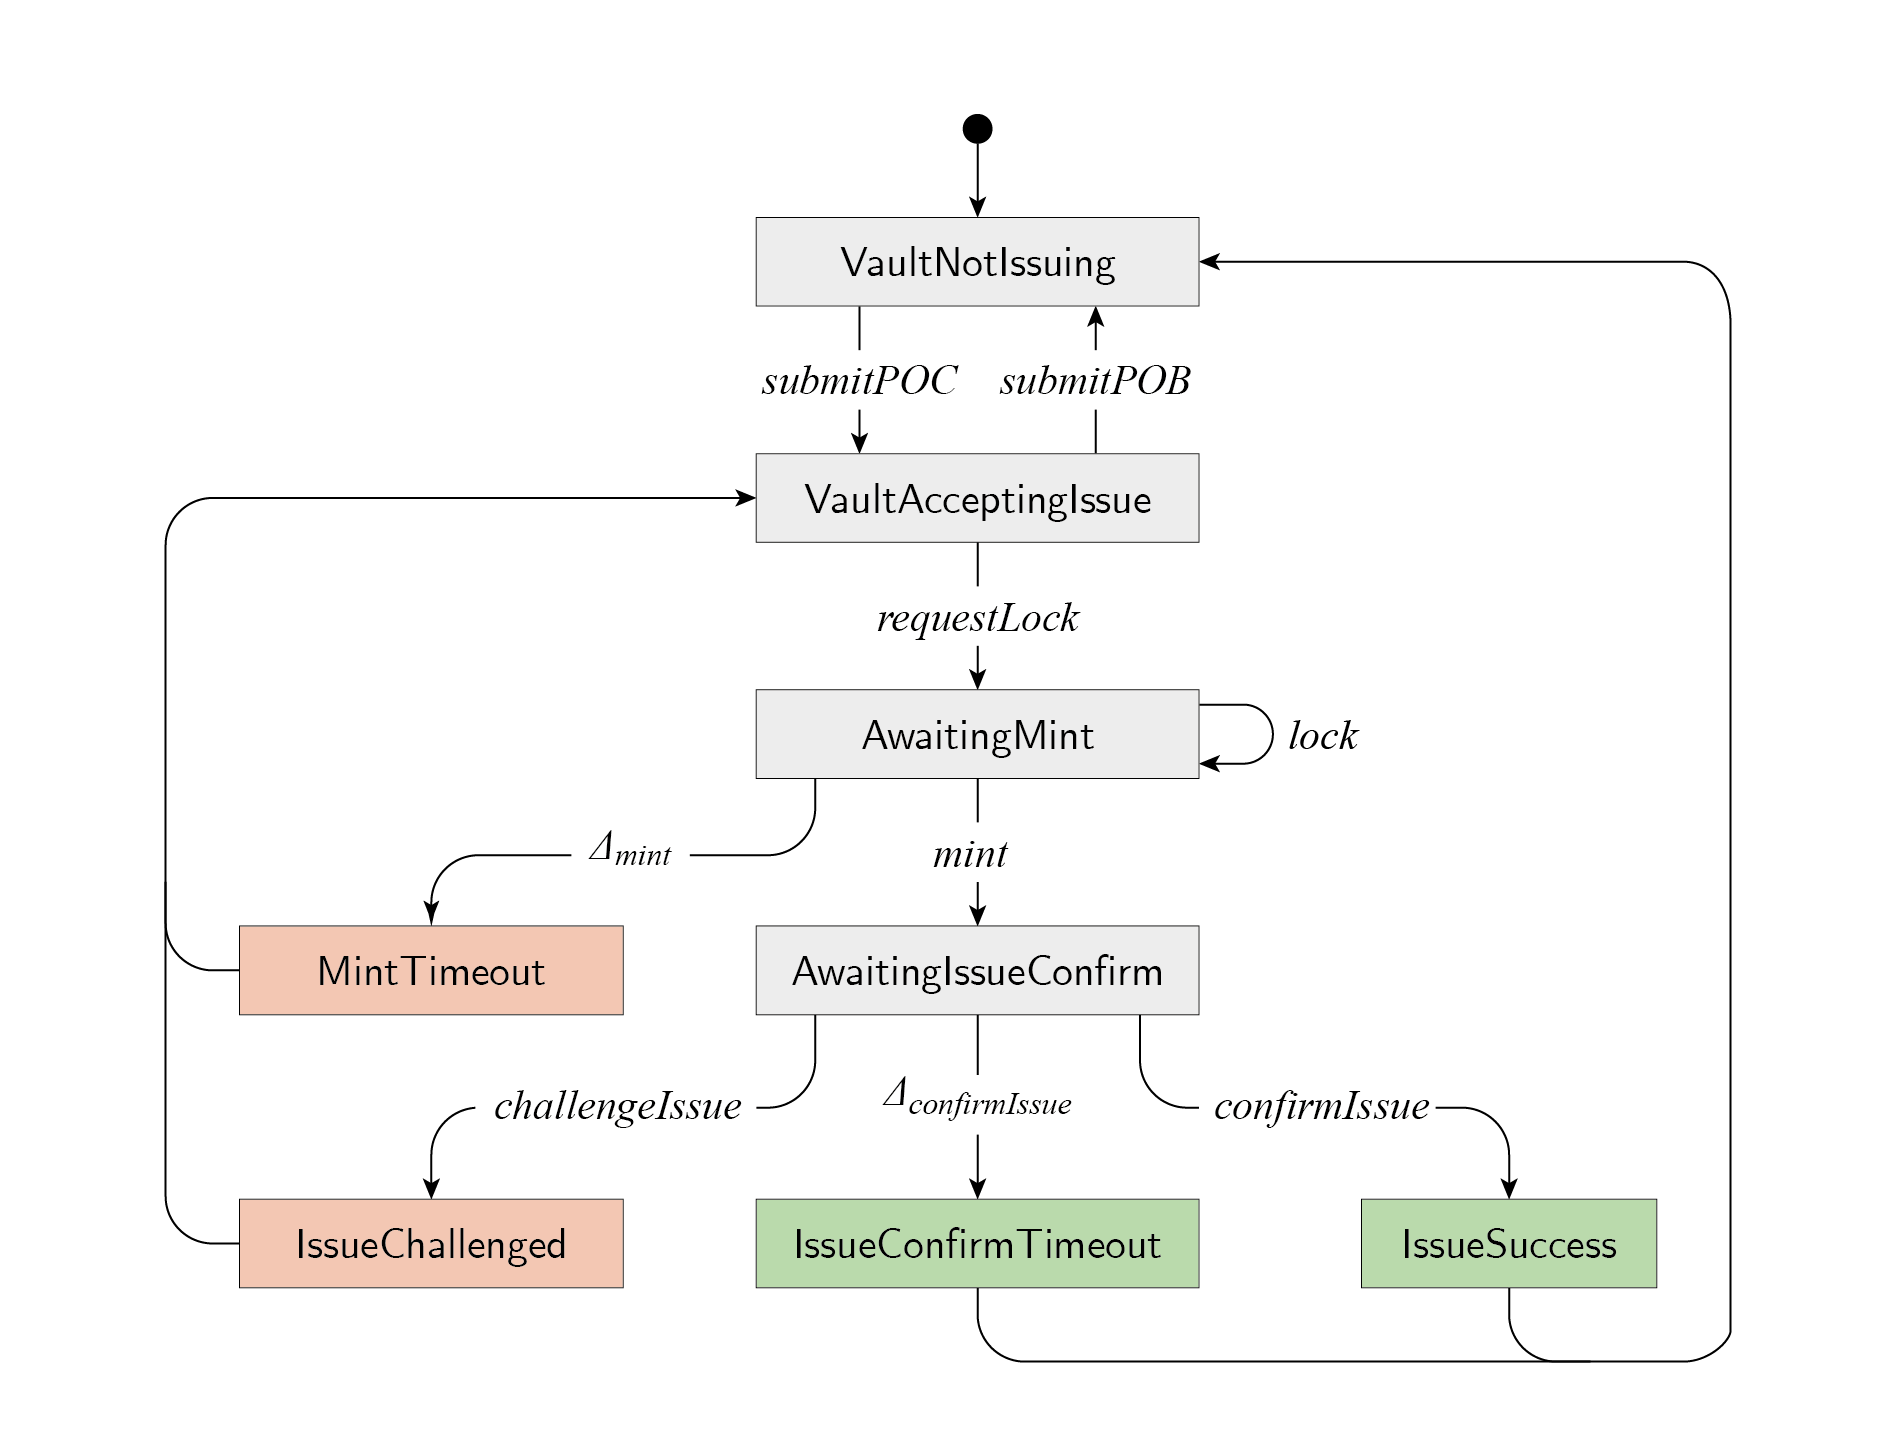
\includegraphics[width=\linewidth]{img/issue.png}
  \caption{Issue}
\end{subfigure}
\begin{subfigure}{\textwidth}
  \centering
  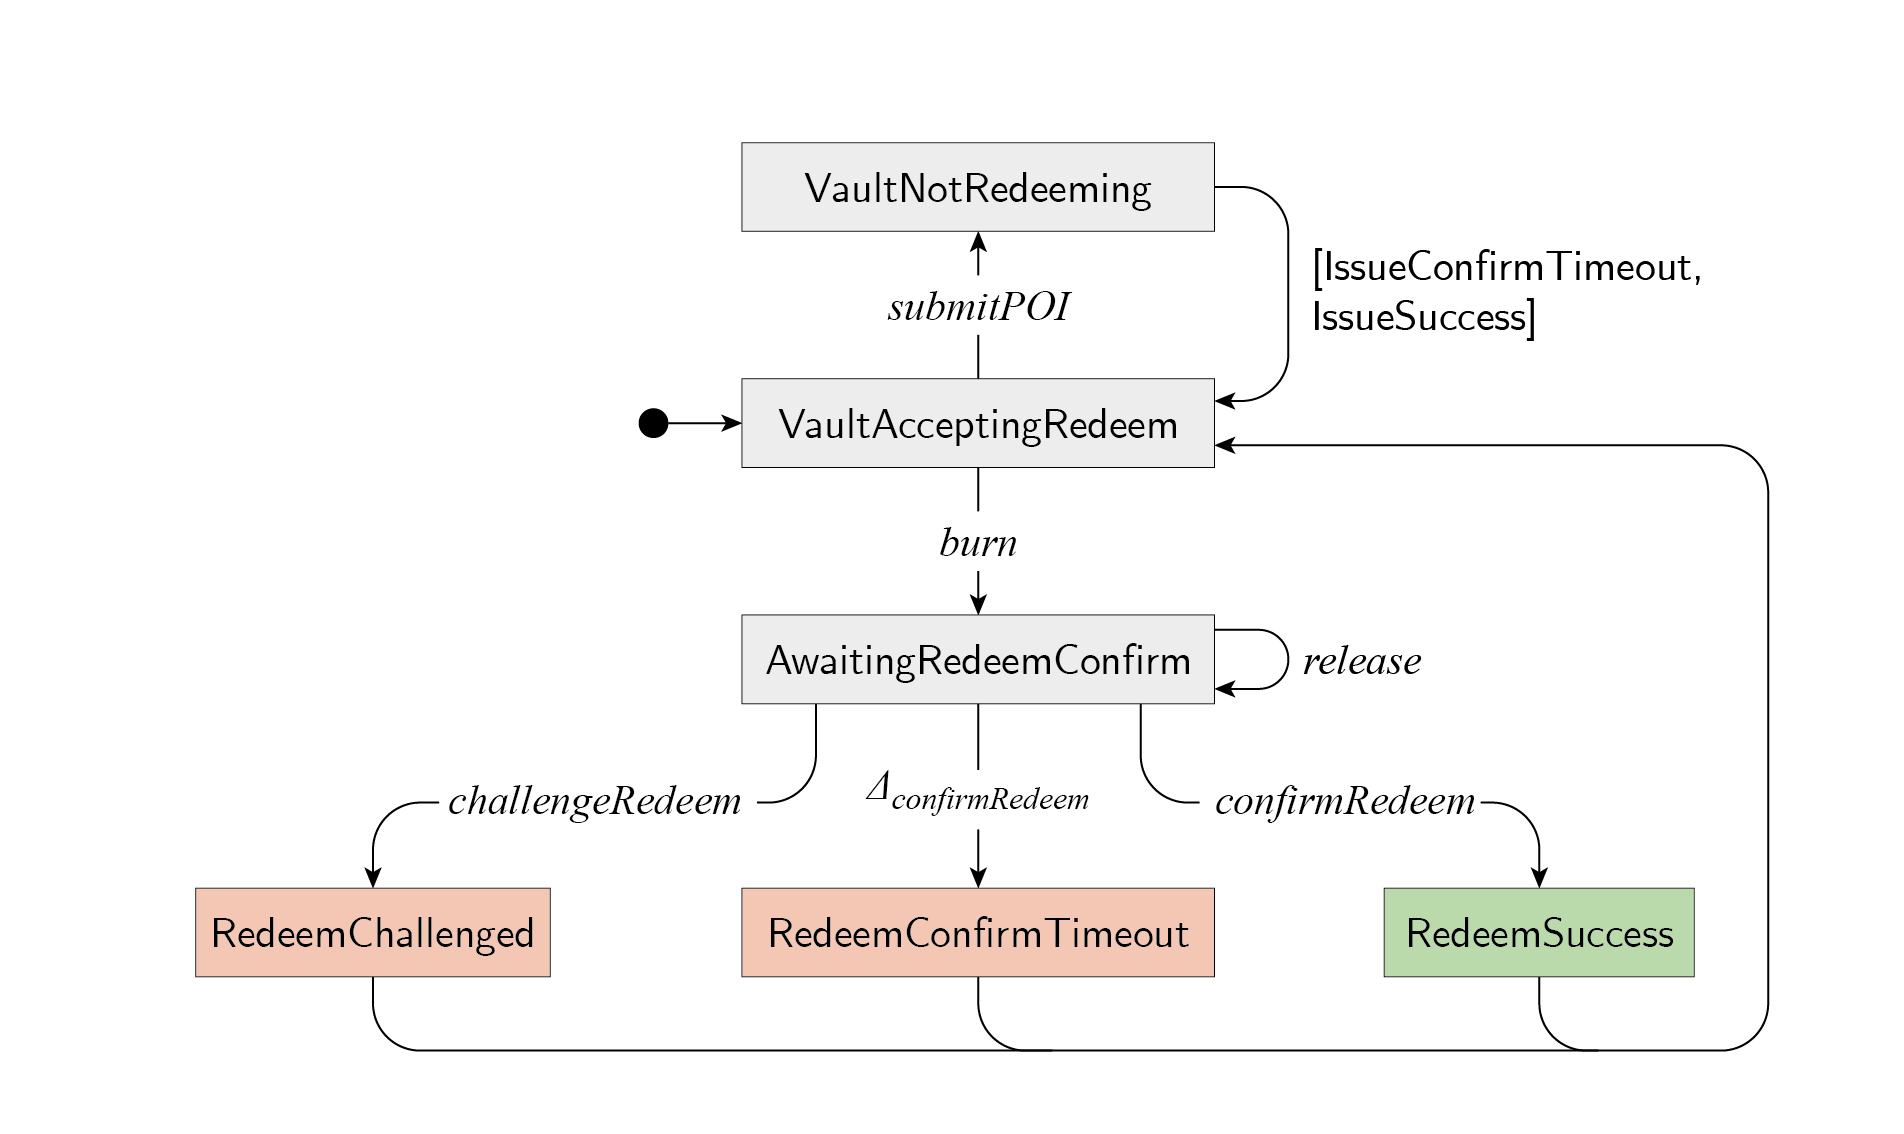
\includegraphics[width=\linewidth]{img/redeem.png}
  \caption{Redeem}
\end{subfigure}
\caption[State diagrams for the Issue and Redeem protocols]{State diagrams for the Issue and Redeem protocols. States colored green represent success, red ones failure.}
\label{fig:state_diagrams}
\end{figure}


\section{Constants}
\label{sec:constants}

The following constants are defined as presented in this section.
Specific values should be chosen following testing and according to implementation constraints.

\begin{itemize}
    \item $\sstd$ is the standard collateralisation ratio.
    
    Vaults periodically provide POBs showing that their collateralisation ratio, i.e.\ the ratio of ZEC obligations to locked collateral according to the exchange rate, is above \sstd.
    Formally, for any vault V:
    \begin{alg}
        \item Let $\vmi$ be the value of the $i$-th \mint transaction in which funds were locked with V, where $0 \leq i \leq n$
        \item Let $\vbj$ be the value of the $j$-th \burn transaction in which funds were released by V, where $0 \leq j \leq m$
        \item Let $\xr_V$ be an exchange rate chosen by the vault, where $\xr_V \leq \xr_\mathcal{O}$, the latest exchange rate provided by the oracle.
        \item Let $\coll$ be the vault's locked collateral.
    \end{alg}

    Then, a proof of balance allows a vault to prove in zero knowledge that
    \begin{equation}\label{eq:coll_pob}
        (\sum_{i=1}^{n} \vmi - \sum_{j=1}^{m} \vbj \cdot \xr_V \cdot \sstd \leq \coll
    \end{equation}
    holds.

    Similarly, in proofs of capacity vaults prove that this inequality holds for their future balance after a lock transaction, regardless of its value.
    See \cref{sec:balance_statements} for more details.
    
    $\sstd$ must be of the form $\frac{p}{q}$, where $p, q \in \N$ and $q$ is a power of 2, in order to make computations in zk-SNARKs in which $\sstd$ is used more efficient.
    
    A suitable value may be $\sstd = \frac{3}{2} = 1.5$.
    
    This value does not need to be a constant but can instead be adjusted on a per-participant basis, where vaults with a trustworthy track record can move up in a tiered system, in order to minimise the opportunity cost due to over-collateralisation~\cite{harz2019balance}.
    
    \item $\smin$ is the minimum collateralisation ratio.
    
    Keeping in mind that the amount of ZEC obligations associated with a vault, $ZEC^{obl} = \sum_{i=1}^{n} v_{l,i} - \sum_{j=1}^{m} v_{r,j}$, is hidden, we can say that vaults provide an upper bound $ZEC^{obl}_\mx$ for this value in \cref{eq:coll_pob}, where $ZEC^{obl}_\mx = \frac{coll}{xr_V \cdot \sstd}$.
    We now define a vault's observed collateralisation ratio $\sigma_{V} = \frac{coll}{xr_t \cdot ZEC^{obl}_\mx}$ as the resulting lower bound on the collateralisation ratio assuming $ZEC^{obl} = ZEC^{obl}_\mx$, where $xr_t$ is the latest exchange rate provided by the oracle.
    
    In order to ensure that all issued funds are properly collateralised, $\sigma_{V}$ can never fall below 1, which may happen if the exchange rate increases by a certain margin.
    Hence we define the minimum collateralisation ratio $\smin$, where $1 < \smin < \sstd$, as the liquidation trigger, i.e.\ liquidation is triggered on vault V whenever $\sigma_{V} \leq \smin$.
    See \cref{sec:liquidation} for more details on liquidation.
    
    For example, $\smin = \frac{9}{8} = 1.125$.
    
    \item \vmax is the maximum value of an issue or redeem transaction in zatoshis, Zcash's smallest unit of currency.
    
    Specifically, this is the maximum amount of funds that can be locked or burned per transaction, i.e.\ prior to the subtraction of fees.
    This limit exists in order to protect the user's privacy, as otherwise amounts in the upper tail of the distribution of Zcash transaction values are more easily identifiable even if the splitting strategy described in \cref{sec:splitting_strategy} is employed.
    
    As argued in the aforementioned section, this value is a power of 2.
    
    \item \vmin is the minimum value of an issue or redeem transaction in zatoshis, i.e.\ the minimum amount of funds that can be locked or burned per transaction.
    
    This lower bound is defined such as to limit the number of transactions resulting from the splitting strategy.
    Besides, sending very small amounts through \zclaim is economically unprofitable as the incurred fees grow larger in proportion to the amount being transferred as the latter decreases, due to the rounding error when computing fees paid to vaults and to transaction fees on Zcash and the issuing chain.
    
    This value is also a power of 2 as per the splitting strategy.
    
    \item $f = \frac{f_n}{f_G}$, where $f_n \in \N$ and $f_G = 2^{\lf}$, represents the fraction of a transaction that goes towards the payment of fees to the vault involved.
    The fee granularity $f_G$ must be a power of two in order to facilitate efficient multiplication in zk-SNARKs.
    \zclaim's fee policy is described in detail in \cref{sec:fees}.
    
    For example, $f = \frac{1}{256}$, which is along the lines of \cba issuing fees in existing protocols~\cite{RenBridgeFAQDarknodes-2020-12-08,WrappedBitcoinWBTCCoinList}.
    
    \item \dm is the mint timeout.
    
    This is the delay from inclusion in $I$ of a lock request to the moment it is discarded if no associated Mint transfer is submitted.
    
    The value \dm is lower bounded by $\Delta^I + \Delta^Z + \Delta_{submit}$, i.e.\ the time the issuer must wait until their lock request and subsequent lock transaction are securely included in $I$ and Zcash, respectively, and the lock transaction can be confirmed by the relay system.
    
    \item \dci is the issue confirmation timeout.
    
    This is the delay within which a vault must confirm the reception of the note in an issuer's lock transfer after the latter has submitted a \mint transaction.
    At the same time, it is the delay within which they may challenge the issuer's \mint transaction if the encryption of the note was erroneous.

    $\Delta_{confirmIsssue}$ may be quite small, as the vault does not need to wait until a \mint transaction is securely included in $I$ to provide confirmation.
    
    
    \item \dcr is the redeem confirmation timeout.
    
    This is the delay within which a vault must confirm the release of funds after a redeemer has submitted a \burn transaction on $I$.
    At the same time, it is the delay within which they may challenge the redeemer's \burn transaction if the encryption of the requested note was erroneous.

    \dcr is lower bounded by $\Delta^I + \Delta^Z + \Delta_{submit}$, i.e.\ the time the vault must wait until the \burn transaction and their release transaction are securely included in $I$ and Zcash, respectively, and the release transaction can be confirmed by the relay system.
    
    In practice, a shorter delay $\dlt{challengeRedeem}$ may be defined within which the vault can challenge the \burn transaction, as they may do so as soon as it is included in $I$, but we choose not to do so for simplicity.
    
    \item \iw is the warranty collateral.
    This is a small amount of collateral that issuers must lock for the duration of an Issue procedure in order to prevent griefing attacks, in which an attacker submits multiple requests to lock funds with vaults without following through.
    Similarly, redeemers must lock this amount when submitting a \burn transaction such as to prevent spam attacks, in which they repeatedly request to redeem but do not properly encrypt the requested note to the vaults.
    
    This amount is also deducted from a vault's collateral if they fail to react in time at any step of the protocols.
    
    \item \lf is the logarithm with base 2 of the fee granularity, as defined for $f$.
    
    \item \lvalueI is defined assuming that the largest possible ICN value can be represented as $ICN_{\max} = 2^{\lvalueI}-1$.
    
    \item $\xr_G$ is the exchange rate granularity.
     Exchange rates on \zclaim are always represented as $\frac{\xr_n}{\xr_G}$.
    
    \item \lxrG is defined such that $\xr_G = 2^{\lxrG}$.

    \item \lxrn is the bit length of the exchange rate numerator such that $\xr_n : \{0\,..\,2^{\lxrn}-1$.
    This value should be chosen such that $\frac{2^{\lxrn}-1}{2^{\lxrG}}$ is large enough to represent a maximum exchange rate above which the protocol collapses, as discussed in \cref{sec:black_swan}.
\end{itemize}


\section{Data structures}

\subsection{Vault representation on \texorpdfstring{$I$}{I}}
A vault V is represented in the vault registry on $I$ by the tuple $(\dvf,\, \pkd,\, \coll,\, \cb,\, \xr_n,\, \acci,\, \accr)$, where
\begin{itemize}
    \item $(\dvf : \B^{[\ld]},\, \pkd : \kas.\ppo)$ is V's diversified payment address on Zcash as provided by themselves upon registration.
    \item $\coll : \{0\,..\,2^{\lvalueI}-1\}$ is the amount of collateral in ICN that V has locked on $I$.
    \item $\cb : \vcm.\out$ is a value commitment to the amount of ZEC obligations associated with V.
    This value is calculated by aggregating the homomorphic value commitments to the ICZ value of all Mint and Burn transfers in which V was involved, employing the abelian group operation on public keys defined in~\cite[Section 4.1.6.2]{hopwood2016zcash} as instantiated for \redjj\footnote{For Burn transfers, the value $-\cv$ where $-\cv + \cv = \mathcal{O}_+$, the group identity, is used instead of \cv.}.
    \item $\xr_n : \{0\,..\,2^{\lxrn}-1$ is the last exchange rate nominator used by the vault in a proof of balance.
    This is used to trigger liquidation when the exchange rate provided by the oracle drops by a certain margin below $\frac{\xr_n}{\xr_G}$.
    \item $\acci : \B$ represents whether V is available to issue funds, i.e.\ accepts lock transactions, where $1 := \top$ and $0 := \bot$.
    \item $\accr : \B$ represents whether V is available to redeem funds, i.e.\ can submit release transactions, where $1 := \top$ and $0 := \bot$.
\end{itemize}

\subsection{Lock permits}
A lock permit is represented as $(\emk, \dvf, \pkd, \nlock)$, where
\begin{itemize}
    \item $\emk : \mas.\pub$ is an ephemeral issuing public key provided by the issuer.
    \emk is a Jubjub public key.

    \item $(\dvf : \B^{[\ld]}, \pkd : \kas.\ppo)$ is the vault's diversified payment address as defined in \cref{sec:zcash_addr}.
    
    \item $\nlock : \By^{[32]}$ is a cryptographic nonce.
    This is the digest of a BLAKE2b-256 hash.
\end{itemize}

\subsection{Mint transfers}
\label{sec:mint_transfers}
A Mint transfer is similar to a Spend transfer in that it allows the issuer to spend some value \val, but instead of proving ownership of a note of this value on $I$, the issuer is required to show that they have locked an equivalent amount of funds on Zcash.
It consists of $(\cv,\, \cvn,\, \crem,\, \emk,\,\, \dvf,\, \pkd,\, \nlock,\, \cmun,\, \posn,\, \rtn,\, \pthn,\, \epkn,\, \cencn,\, \sig,\, \pim)$, where:
\begin{itemize}
    \item $\cv : \vcm.\out$ is a commitment to the ICZ value $\val$ being minted.
    
    \item $\cvn : \vcm.\out$ is a commitment to the ZEC value $\valn$ that the issuer has locked with the vault on Zcash.
    
    \item $\crem : \vcm.\out$ is a commitment to the fee rounding error.
    This value is used to verify that the relation between $\val$ and $\valn$ holds based on the value commitments \cv and \cvn.
    
    \item $\emk : \mas.\pub$ is the minting public key in the lock permit allowing the issuer to lock funds with this vault.
    
    \item $(\dvf : \B^{[\ld]}, \pkd : \kas.\ppo)$ is the vault's shielded payment address in the lock permit.
    
    \item $\nlock : \By^{[32]}$ is the nonce in the lock permit.
    
    \item $\cmun : \B^{[\lms]}$ is the note commitment hash of the note the issuer sent to the vault.
    
    \item $\posn : \{0\,..\,2^{\mds} - 1\}$ is the position of \cmun in the note commitment tree.
    
    \item $\rtn : \B^{[\lms]}$ is an anchor for the output treestate of a Zcash block.
    
    \item $\pthn : (\B^{[\lms]})^{[\mds]}$ is a Merkle path as defined in~\cite[Section 4.8]{hopwood2016zcash} from \cmun to \rtn.
    
    \item $\epkn : \kas.\pub$ is the ephemeral key agreement public key used to derive the key for the encryption of the transmitted note ciphertext component \cencn.
    
    \item $\cencn : \symc$ is the encrypted note plaintext $(\dvf, \val, \rcm, \memo)$ of the note with note commitment $\cmun$ encrypted as defined in~\cite[Section 4.17.1]{hopwood2016zcash}.
    The vault needs the values \dvf, \v, \rcm in order to be able to spend the aforementioned note.
    The \memo field is irrelevant to the \zclaim protocol.
    
    \item $\sig : \mas.\signature$ is a signature over the \sighash transaction hash that must be verifiable using $\emk$.
    
    \item $\pim : \zkm.\proof$ is a \groth zk-SNARK with primary input $(\cv, \cvn, \crem, \gdstar, \pkdstar, \nlock, \cmun)$, where $\gdstar = \reprj(\divhash(\dvf))$ and $\pkdstar = \reprj(\pkd)$.
    \pim is a proof for a Mint statement, defined in \cref{sec:mint}.
\end{itemize}

\subsection{Burn transfers}
\label{sec:burn_transfers}
Similarly, a Burn transfer is similar to an Output transfer.
As the name suggests, it allows a redeemer to burn assets and redeem their value on Zcash.
It consists of $(\cv, \cvn, \crem, \dvf, \pkd, \cmun, \epk, \nenc, \pib)$, where:
\begin{itemize}
    \item $\cv : \vcm.\out$ is a commitment to the ICZ value $\val$ being burned.
    
    \item $\cvn : \vcm.\out$ is a commitment to the ZEC value $\valn$ that the redeemer requests the vault to release.

    \item $\crem : \vcm.\out$ is a commitment to the fee rounding error.
    This value is used to verify that the relation between $\val$ and $\valn$ holds based on the value commitments \cv and \cvn.
    
    \item $(\dvf : \B^{[\ld]}, \pkd : \kas.\ppo)$ represent the vault the redeemer is requesting to release funds.
    
    \item $\cmun : \B^{[\lms]}$ is the note commitment hash of the note the redeemer requests to receive on Zcash.
    
    \item $\epk : \kas.\pub$ is the ephemeral key agreement public key used to derive the key for the encryption of the note with note commitment \cmun to the vault.
    
    \item $\nenc : \symc$ is encryption of the note values of the note with note commitment $\cmun$ as defined in~\cite[Section 4.17.1]{hopwood2016zcash}, where the note plaintext \np is simply replaced by the note \n.
    
    \item $\pib : \zkb.\proof$ is a \groth zk-SNARK with primary input $(\cv, \cvn, \crem, \cmun)$ for a Burn statement, defined in \cref{sec:burn}.
\end{itemize}


\section{Issuing}
\label{sec:issuing}

We now provide a specification for the Issue protocol based on the operations introduced in previous sections.
For each operation, we define pre-execution steps, a transaction, requirements for that transaction to succeed, and the outcome in case of success.
We define the protocol between two actors: an issuer \issuer and a vault \vault.

\subsection{\requestLockop}

\paragraph{Pre-execution steps}
\issuer queries the vault registry for a vault available to issue, i.e.\ for which $\acci = \top$.
They generate a \mas private/public key pair $(\emsk : \mas.\priv,\, \emk.\pub)$ as follows:
\begin{alg}
    \item Let \mas be the signature scheme defined in \cref{app:mas}
    \item Let $\emsk = \mas.\genp$
    \item Let $\emk = \mas.\derivepub(\emsk)$
\end{alg}

\paragraph{Transaction}
\issuer submits a \requestLock transaction on $I$, which locks \iw and takes $(\emk, \dvf, \pkd, \rlsig)$ as input, where
\begin{itemize}
    \item $\emk : \mas.\pub$ is the public component of the key pair generated by \issuer.

    \item $(\dvf : \B^{[\ld]},\, \pkd : \kas.\ppo)$ is the diversified payment address of the vault \vault selected by the issuer.
    
    \item $\rlsig : \mas.\signature$ is a signature over this transaction, computed as follows:
    \begin{alg}
        \item Let \rlhash be the digest of an unspecified hash function on the canonical encodings of all other fields in this transaction.
        \item Then, $\rlsig = \mas.\sign_{\emsk}(\rlhash)$
    \end{alg}
\end{itemize}

\paragraph{Requirements}
A \requestLock transaction is successful if:
\begin{itemize}
    \item \issuer's ICN balance is larger than \iw.
    \item $\acci = \top$ for vault \vault with diversified payment address $(\dvf, \pkd)$.
    \item $\emk$ has not been used in a previous \requestLock transaction in this block.
    \item $\mas.\validate_{\emk}(\rlhash, \rlsig) = 1$.
\end{itemize}

\paragraph{Outcome}
$\acci$ is set to $\bot$ for \vault and a lock permit is issued containing $(\emk, \dvf, \pkd, \nlock)$, where
\begin{itemize}
    \item $\emk, \dvf, \pkd$ are the values submitted by \issuer in the \requestLock transaction.
    \item $\nlock$ is a cryptographic nonce that \issuer must use to derive the note commitment trapdoor in the note they send to \vault. This value is generated as follows:
    \begin{alg}
        \item Let \prevheader be the concatenation of the encoding of all fields in the previous block header on $I$, i.e.\ the header of the block immediately preceding the one in which the lock permit is to be included.
        \item Then, $\nlock = \blakezclaim(\text{``\zclaimnl''}, \prevheader\\ \;||\; \emk)$
    \end{alg}
    
    Since it is verified that no two ephemeral issuing keys in lock requests in the same block are the same, this value is unique.
\end{itemize}

If \issuer does not submit a \mint transaction within \dm, the lock permit is discarded and \issuer's warranty collateral \iw is transferred to \vault.

\subsection{\lockop}
\label{sec:lock}

\paragraph{Pre-execution steps}
\issuer waits until the preceding \requestLock transaction is securely included on $I$.
They craft a note \n to send to \vault with destination diversified payment address $(\dvf, \pkd)$, value $\valn \leq \vmax$ and note commitment trapdoor \rcmn generated as follows:
\begin{alg}
    \item Let \nncm be the nonce commitment scheme defined in\\ \cref{app:nncm}
    \item Choose a uniformly random nonce commitment trapdoor $\rcn \xleftarrow{\text{R}}\\ \nncm.\gent$
    \item Then, $\rcmn = \nncm_{\rcn}(\nlock)$
\end{alg}

\paragraph{Transaction}
The \lock transaction that \issuer must submit on Zcash may be any transaction in which \n is the output note of an Output transfer.
We call this Output transfer the lock transfer.
Besides, the \lock transaction may contain any number of transparent inputs and outputs, Spend transfers and other Output transfers.

\paragraph{Requirements}
The \lock transaction succeeds if it follows the standard Zcash protocol rules.
See the specification for more details.

\paragraph{Outcome}
This transaction has no immediate effect on $I$.

\subsection{\mintop}
\label{sec:mint}

\paragraph{Pre-execution steps}
\issuer waits until the \lock transaction has been securely included on Zcash and confirmed by the relay system.

They calculate the ICZ value to be minted after deduction of fees as $\val = \left \lfloor{\valn \cdot (1 - f)}\right \rfloor$ and construct a Mint transfer as defined in \cref{sec:mint_transfers} using the following values:
\begin{itemize}
    \item $\cv$ must be a value commitment to the ICZ value being minted, in which the randomness must be derived from the note commitment trapdoor of note \n as follows:
    \begin{alg}
        \item Let $\rcv =\\ \leostoip_{256}(\blakezclaim(\text{``\zclaimcv''}, \rcmn)) \mod 2^{251}$
        \item Then, $\cv = \vcm_{\rcv}(\val)$
    \end{alg}
    
    \item $\cvn$ is a value commitment for $\valn$, the ZEC value locked with \vault.
    Generally, this will be the value commitment \cv in the lock transfer.
    Otherwise, it is to be generated in the same way as the aforementioned as described in~\cite[Section 4.6.2]{hopwood2016zcash}, i.e.:
    \begin{alg}
        \item Choose a uniformly random commitment trapdoor $\rcvn \xleftarrow{\text{R}}\\ \vcm.\gent$
        \item Then, $\cvn = \vcm_{\rcvn}(\valn)$
    \end{alg}

    \item $\crem$ is a value commitment to the fee rounding error.
    This value must be computed as $\crem = [f_G]\,\cv - [f_G - f_n]\,\cvn$.
    
    \item $\emk, \dvf, \pkd, \nlock$ are the values in the lock transfer.
    
    \item $\cmun$ must be the note commitment hash of note \n, generated as described in~\cite[Section 4.6.2]{hopwood2016zcash} as follows:
    \begin{alg}
        \item Let $\gd = \divhash(\dvf)$
        \item Then, $\cmun = \extractj(\ncm[\rcmn](\reprj(\gd), \reprj(\pkd), \valn))$
    \end{alg}
    This value is published in the lock transfer, at which point it is added to Zcash's note commitment tree.
    
    \item $\posn$ is the index of the leaf node occupied by the hash value \cmun in Zcash's note commitment tree.
    This value is obtained by examining the note commitment tree after the lock transaction has been included in a block.
    
    \item \rtn must be an anchor for the output treestate of a Zcash block of block height $h \geq h_\n$, where $h_\n$ is the height of the block in which \n was created.
    
    \item $\pthn$ is a Merkle path from the leaf node containing $\cmun$ to \rtn, generated as described in~\cite[Section 4.8]{hopwood2016zcash}.
    
    \item $\epkn$ is used in the symmetric encryption scheme used to encrypt and decrypt \cencn.
    
    Generally, this will be the value \epk used in the lock transfer.
    Otherwise, it is to be generated in the same way as \epk as described in~\cite[Sections 4.6.2 and 4.17.1]{hopwood2016zcash}, i.e.:
    \begin{alg}
        \item Choose a uniformly random ephemeral private key\\ $\eskn \xleftarrow{\text{R}} \kas.\priv \backslash \{0\}$
        \item Then $\epkn = \kas.\derivepub(\eskn, \divhash(\dvf))$, where \dvf is \vault's diversifier
    \end{alg}

    \item $\cencn$ is the note plaintext of note \n encrypted as defined in~\cite[Section 4.17.1]{hopwood2016zcash}.
    
    Generally, this will be the value $\cenc$ in the lock transfer.
    Otherwise, it is to be generated in the same way as \cenc as described in~\cite[Section 4.17.1]{hopwood2016zcash} with $\esk = \eskn$, the private key from which \epkn was derived.
    
    \item $\sig$ is generated as follows:
    \begin{alg}
        \item Let \sighashvar be the \sighash transaction hash as defined in \cref{app:sighash}
        \item Then, $\sig = \mas.\sign_{\emsk}(\sighashvar)$, where \emsk is the private key from which \emk was derived
    \end{alg}
    
    \item $\pim$ is a zero-knowledge proof for a Mint statement, which proves that, given a primary input
    \begin{alignat*}{2}
        (&\cv      &&: \vcm.\out,\\
         &\cvn     &&: \vcm.\out,\\
         &\crem    &&: \vcm.\out,\\
         &\gdstar  &&: \B^{[\lj]},\\
         &\pkdstar &&: \B^{[\lj]},\\
         &\nlock   &&: \By^{[32]},\\
         &\cmun    &&: \B^{[\lms]}),
    \intertext{the prover knows an auxiliary input}
        (&\val     &&: \{0\,..\,\vmax\},\\
         &\valn    &&: \{0\,..\,\vmax\},\\
         &\rcvn    &&: \{0\,..\,2^{\lscalar}-1\},\\
         &\rcmn    &&: \{0\,..\,2^{\lscalar}-1\},\\
         &\rcnn    &&: \{0\,..\,2^{\lscalar}-1\},\\
         &\rcv     &&: \{0\,..\,2^{\lscalar}-1\},\\
         &\rcr     &&: \{0\,..\,2^{\lscalar}-1\},\\
         &\rem     &&: \{0\,..\,f_G-1\})
    \end{alignat*}
    such that the following conditions hold:
    
    \textbf{Note commitment integrity}\\
    $\cmun = \extractj(\ncm[\rcmn](\gdstar, \pkdstar, \valn))$
    
    \textbf{Locked value commitment integrity}
    $\cvn = \vcm_{\rcvn}(\valn)$
    
    \textbf{Minted value commitment integrity}
    $\cv = \vcm_{\rcv}(\val)$
    
    \textbf{Fee rounding commitment integrity}
    $\crem = \vcm_{\rcr}(\rem)$
    
    \textbf{Trapdoor commitment integrity}
    $\rcvn = \nncm_{\rcnn}(\nlock)$
    
    Apart from these constraints, all auxiliary inputs must be range checked and some small order checks may be necessary.
    
    \medskip
    The purpose of the \textbf{Trapdoor commitment integrity} condition is to ensure that note \n was created expressly for the purpose of this Issue procedure.
    Alternatively, a collection containing positioned Zcash notes used in past Issue procedures could be implemented on $I$, which would however lead to a larger strain on storage and computational power due to the insertion and searching of notes in this data structure.
    
    The concrete implementation of this zk-SNARK falls beyond the scope of this work, but the above conditions have been chosen such that they can be implemented using circuit components already in use in the Sapling zk-SNARKs, as per the stated \textbf{Minimal modifications} design goal.
    
    \medskip
    \issuer instantiates this zk-SNARK with auxiliary inputs $\rcr = f_G \cdot \rcv - (f_G - f_n) \cdot \rcvn$ and $\rem = f_G \cdot \val - (f_G - f_n) \cdot \valn$, primary inputs $\gdstar = \reprj(\divhash(\dvf))$ and $\pkdstar = \reprj(\pkd)$ and all other values as previously defined.
\end{itemize}

\paragraph{Transaction}
A \mint transaction is a transaction on $I$ that contains a Mint transfer and any number of transparent inputs and outputs, and Spend and Output transfers.
Ideally, however, it should only contain Spend and Output transfers apart from the Mint transfer, such as not to compromise privacy.
See discussion in \cref{sec:privacy} on the matter.
Usually, it will consist of only the Mint transfer and one Output transfer.

\issuer submits a \mint transaction on $I$ containing the Mint transfer described above.

\paragraph{Requirements}
The \mint transaction succeeds only if the following conditions hold for the Mint transfer:
\begin{itemize}
    \item \pthn is a Merkle path from \cmun to \rtn.
    This is verified as follows:
    \begin{alg}
        \item Let $\hash_{\mds} = \cmun$
        \item Let $\pth[i]$ be the $i$-th element of the Merkle path, where $0 \leq i \leq \mds - 1$
        \item For $i$ from $\mds$ down to 1:
        \begin{alg}
            \item Let $\parity = \left \lfloor{\frac{\posn}{2^{\mds - i}}}\right \rfloor \,\&\, 1$
            \item Let $\hashvar = \hash_{i}$
            \item Let $\sib = \pth[\mds - i]$
            \item If $\parity = 0$:
            \begin{alg}
                \item Let $\hash_{i-1} = \mcrh(i - 1,\, \hashvar,\, \sib)$
            \end{alg}
            \item Else:
            \begin{alg}
                \item Let $\hash_{i-1} = \mcrh(i - 1,\, \sib,\, \hashvar)$
            \end{alg}
        \end{alg}
        \item Then, return $\top$ if $\hash_{0} = \rtn$ and $\bot$ otherwise
    \end{alg}

    \item \rtn is an anchor for the output treestate of a Zcash block that has been confirmed by the relay system.
    In Sapling, \rtn is encoded in block headers as the field \hfsr.
    
    As a side note, this field was replaced with a commitment to a larger data structure that in turn commits to the note commitment tree~\cite{zipszip0221flyclient} in the recent Heartwood upgrade~\cite{HeartwoodZcash} mentioned in \cref{sec:verification_size}.
    This data structure is a Merkle Mountain Range (MMR) that also commits to several other features of the chain's history.
    Hence, showing that \rtn is indeed an anchor for the output treestate of a post-Heartwood block would imply providing a path from \rtn to the root of the MMR.

    \item The values $\emk, \dvf, \pkd, \nlock$ match those in a lock permit.
    
    \item The relation
    \begin{equation}\label{eq:cr}
        \crem = [f_G]\,\cv - [f_G - f_n]\,\cvn
    \end{equation}
    holds.
    
    As per the specification of \vcm in~\cite[Section 5.4.7.3]{hopwood2016zcash}, this expands to
    \begin{align*}
        \crem &= [f_G]\, ([\val]\, \mathcal{V} + [\rcv]\, \mathcal{R}) - [f_G - f_n]\, ([\valn]\, \mathcal{V} + [\rcvn]\, \mathcal{R})\\
        &= [f_G \cdot \val - (f_G - f_n) \cdot \valn]\, \mathcal{V} + [f_G \cdot \rcv - (f_G - f_n) \cdot \rcvn]\, \mathcal{R}\\
        &= [\rem']\, \mathcal{V} + [\rcr']\, \mathcal{R}\\
        &= \vcm_{\rcr'}(\rem')
    \end{align*}
    Since \pim proves that $\crem = \vcm_{\rcr}(\rem)$ for some $\rem < f_G$, it follows from \cref{eq:cr} and the security requirements of \vcm, which must be computationally binding, that
    \begin{gather*}
        f_G \cdot \val - (f_G - f_n) \cdot \valn = \rem' = \rem \leq f_G\\
        \Leftrightarrow \quad \val = \left \lfloor{\valn \cdot (1 - f)}\right \rfloor
    \end{gather*}
    
    Hence this check ensures that the minted value was calculated correctly.
    The verification is done outside of \pim for efficiency reasons.

    \item \pim is verified to be correct as described in~\cite[Appendix B.2]{hopwood2016zcash}.
    
    \item $\mas.\validate_{\emk}(\sighashvar, \sig) = 1$.
\end{itemize}

\paragraph{Outcome}
This operation creates a \mint transaction that is published but not included in the block chain until either \vault executes \confirmIssueop or the delay \dci has passed.
If \vault executes \challengeIssueop within said delay, the transaction is discarded.

If no \confirmIssue or \challengeIssue transaction is submitted within this delay, the outcome is still the same as that of a \confirmIssue operation, but additionally, \iw is deducted from \vault's collateral and transferred to \issuer.
In that case, we assume that \issuer has no way of knowing in advance that \vault will not be able to react and thus must have encrypted the note plaintext correctly.

The corresponding lock permit is immediately discarded.

\subsection{\confirmIssueop}
\label{sec:confirm_issue}

\paragraph{Pre-execution steps}
\vault sees the pending \mint transaction on $I$ containing a Mint transfer that includes their diversified payment address \dpa.
They proceed to verify the validity of said Mint transfer as follows:
\begin{enumerate}
    \item \textbf{Note ciphertext verification.}
    
    If \vault has received the note plaintext of note \n with note commitment \cmun in the lock transaction, they can skip this step.
    
    Otherwise, they decrypt \cencn as described in~\cite[Section 4.17.2]{hopwood2016zcash} with parameters \ephkey, \cenc and $\mathtt{cmu}$ being the encodings of \epkn, \cencn and \cmun, respectively.
    There is no need to verify that \vault is the recipient of the note as this is already proven in the zk-SNARK.
    
    \item \textbf{Value commitment randomness verification.}
    
    \vault needs to know the trapdoor used to generate the value commitment \cv in the Mint transfer in order to be able to submit proofs of balance including said transfer.
    
    Hence they verify that the trapdoor was derived from \n's note commitment trapdoor as follows:
    \begin{alg}
        \item Let \rcmn and \valn be the note commitment trapdoor and value in the decrypted note plaintext \np
        \item Let $\val = \left \lfloor{\valn \cdot (1 - f)}\right \rfloor$ be the minted value
        \item Let $\rcv' =\\ \leostoip_{256}(\blakezclaim(\text{``\zclaimcv''}, \rcmn)) \mod 2^{251}$
        \item Let $\cv' = \vcm_{\rcv'}(\val)$
        \item Then, return $\top$ if $\cv = \cv'$, otherwise return $\bot$
    \end{alg}
\end{enumerate}
If any of these steps fails, \vault should execute \challengeIssueop instead.

\paragraph{Transaction}
\vault submits a \confirmIssue transaction on $I$, which takes $(\dvf,\, \pkd,\, \nlock,\, \icsig)$ as input, where:
\begin{itemize}
    \item \dvf, \pkd, \nlock must be the values in the Mint transfer to be confirmed.
    
    \item $\icsig : \vaultsig.\signature$ is a signature over the hashes of this transaction and the Mint transfer, computed as follows:
    \begin{alg}
        \item Let \mhash be a hash of the canonical encoding of all fields in the Mint transfer
        \item Let \cihash be a hash of the canonical encoding of all other fields in the \confirmIssue transaction
        \item Let \ivk be \vault's incoming viewing key
        \item Let \vaultsig be the signature scheme defined in \cref{app:vaultsig}
        \item Then, $\icsig = \vaultsig.\sign_{\ivk}(\cihash \;||\;\allowbreak \mhash)$
    \end{alg}
    
    The input to this signature includes the hash of the Mint transfer since the \confirmIssue transaction may otherwise be replayed over a different Mint transfer in which the note values have not been correctly encrypted to \vault in a double spend attack.
    If \vault has not saved these values when confirming the original transfer, they will not have access to the locked funds.
\end{itemize}

\paragraph{Requirements}
The \confirmIssue transaction succeeds if:
\begin{itemize}
    \item The values $\dvf, \pkd, \nlock$ match those in a pending Mint transfer.
    \item  $\vaultsig.\validate_{\pkd}(\cihash \;||\; \mhash, \icsig) = 1$.
\end{itemize}

\paragraph{Outcome}
The \mint transaction is confirmed and the minted funds become immediately available to \issuer.

The ZEC obligations value commitment \cb associated with \vault is updated as follows:
\begin{alg}
    \item Let $\cv$ be the ICZ value commitment in the Mint transfer
    \item Let `+' be the abelian group operation on public keys defined in~\cite[Section 4.1.6.2]{hopwood2016zcash} as instantiated for \redjj
    \item Then, let $\cb^{\new}$ = $\cb^{\old} + \cv$
\end{alg}

The warranty collateral \iw is returned to \issuer.

\subsection{\challengeIssueop}

\paragraph{Pre-execution steps}
\vault has established the invalidity of the pending Mint transfer as per the pre-transaction steps of \confirmIssueop.

\paragraph{Transaction}
A \challengeIssue transaction on $I$ takes $(\shared,\, \dvf,\, \pkd,\, \epkn,\, \pic)$ as input, where:
\begin{itemize}
    \item $\shared : \kas.\Shared$ is the shared secret presumably used by \issuer to encrypt \cencn.
    This value is computed by \vault as $\shared = \kas.\agree(\ivk, \epkn)$.
    
    \item \dvf, \pkd, \epkn must be the values in the Mint transfer.

    \item $\pic : \pic.\proof$ is a \groth zk-SNARK for a Challenge statement, which proves that, given a primary input
    \begin{alignat*}{2}
        (&\shared &&: \kas.\Shared,\\
         &\gd     &&: \kas.\ppo,\\
         &\pkd    &&: \kas.\ppo,\\
         &\epk    &&: \kas.\pub)
    \intertext{the prover knows an auxiliary input}
        (&\ivk    &&: \{0\,..\,2^{\livk}-1\})
    \end{alignat*}
    such that the following conditions hold:
    
    \textbf{Diversified address integrity}
    $\pkd = [\ivk]\,\gd$
    
    \textbf{Shared secret integrity}
    $\shared = [\hj \cdot \ivk]\,\epk$
    
    \medskip
    Effectively, this statement is a non-interactive proof of discrete-logarithm equality or DLEQ, with input pairs $(\pkd, \gd)$ and $(\shared, [\hj]\,\epkn)$.
    This proof allows \vault to show that the revealed shared secret was correctly generated using their incoming viewing key without revealing the latter.
    
    \vault must instantiate this zk-SNARK with primary inputs $(\shared,\, \divhash(\dvf),\, \pkd,\, \epkn)$.
\end{itemize}

This transaction does not contain a signature since the vault already proves knowledge of their own incoming viewing key \ivk in \pic.
Furthermore, it is not necessary to commit to the Mint transfer since a \challengeIssue transaction may only be replayed over a different Mint transfer if the encryption of \cencn is also erroneous in said transfer, which does not represent undesirable behaviour.

\paragraph{Requirements}
The \challengeIssue transaction succeeds if:
\begin{itemize}
    \item The values \dvf, \pkd, \epkn match those in a pending Mint transfer.
    
    Note that the values \dpa are enough to uniquely identify the Mint transfer, since \zclaim currently only allows for one concurrent Issue procedure per vault.
    If the protocol is expanded to allow multiple concurrent instances of Issue per vault, the value \nlock should be added to the \challengeRedeem transaction inputs as there is no mechanism in place to prevent \epkn from begin reused across multiple Issue transfers.
    \item The verification of \pic as described in~\cite[Appendix B.2]{hopwood2016zcash} succeeds.
    \item Any of \textbf{Note ciphertext verification} or \textbf{Value commitment randomness verification} as defined in the pre-execution steps of \confirmIssueop fail.
    
    This can be verified using the revealed shared secret as follows:
    \begin{alg}
        \item Attempt decryption of \cencn as described in \textbf{Note ciphertext verification}.
        Skip step 3 in~\cite[Section 4.17.2]{hopwood2016zcash} referenced therein and let \shared be the value revealed by \vault in this transaction.
        \item If the decryption algorithm returns $\bot$, return $\top$.
        \item Verify that the trapdoor for \cv was correctly derived as described in \textbf{Value commitment randomness verification}.
        \item If the verification algorithm returns $\bot$, return $\top$. Otherwise return $\bot$.
    \end{alg}
\end{itemize}

\paragraph{Outcome}
The challenged \mint transaction is discarded and \issuer's warranty collateral \iw is paid to \vault to compensate for the opportunity cost.

Note that if the note values were correctly transmitted but \vault successfully challenged the \mint transaction due to an erroneously constructed \cv, \vault retains control over the locked funds.
In order to prevent this situation, issuers should adhere to the protocol.


\section{Redeeming}
\label{sec:redeeming}
Similarly, we define the Redeem protocol between a redeemer \redeemer and a vault \vault.

\subsection{\burnop}
\label{sec:burn}

\paragraph{Pre-execution steps}
\redeemer queries the vault registry for a vault available to redeem, i.e.\ for which $\accr = \top$.
They decide on \vault with diversified payment address \dpa.

\redeemer determines an amount $\val \leq \vmax$ of ICZ to burn and calculates the amount of ZEC that they can request \vault to release after deduction of fees as $\valn = \left \lfloor{\val \cdot (1 - f)}\right \rfloor$.
They construct a Zcash note \n, which \vault will be requested to create, with a destination diversified payment address $(\dvfn, \pkdn)$ of their choice, value \valn and randomly generated randomness \rcmn.

Then, they construct a Burn transfer as defined in \cref{sec:burn_transfers} using the following values:
\begin{itemize}
    \item $\cv$ must be a value commitment to the ICZ value being burned, in which the randomness must be derived from the note commitment trapdoor of note \n in the same way as \cv in Mint transfers.
    
    \item $\cvn$ must be a value commitment to the ZEC value to be released \valn, generated as follows:
    \begin{alg}
        \item Choose a uniformly random commitment trapdoor $\rcvn \xleftarrow{\text{R}}\\ \vcm.\gent$
        \item Then, $\cvn = \vcm_{\rcvn}(\valn)$
    \end{alg}
    
    \item \crem must be a value commitment to the fee rounding error.
    This value is computed as $\crem = [f_G]\,\cvn - [f_G - f_n]\,\cv$.
    
    \item \dpa is \vault's diversified payment address.
    
    \item $\cmun$ is generated as follows:
    \begin{alg}
        \item Let $\gdn = \divhash(\dvfn)$
        \item Then, $\cmun = \extractj(\ncm[\rcmn](\reprj(\gdn), \reprj(\pkdn), \valn))$
    \end{alg}
    
    \item $\epk$ is generated as described in~\cite[Sections 4.6.2 and 4.17.1]{hopwood2016zcash}, i.e.:
    \begin{alg}
        \item Choose a uniformly random ephemeral private key\\ $\esk \xleftarrow{\text{R}} \kas.\priv \backslash \{0\}$
        \item Then $\epk = \kas.\derivepub(\esk, \divhash(\dvf))$, where \dvf is \vault's diversifier
    \end{alg}
    
    \item $\nenc$ is obtained from \n and \val similarly to \cenc from \np in Output transfers:
    \begin{alg}
        \item Let \zcashvar{N} be the canonical encoding of all fields of note \n, i.e.\ $(\dvfn,\, \pkdn,\, \valn,\, \rcmn)$
        \item Let $\ephkey = \lebstoosp_{\lj}(\reprj(\epk))$
        \item Let $\shared = \kas.\agree(\esk, \pkd)$
        \item Let $\kenc = \kdfs(\shared, \ephkey)$
        \item Then, $\nenc = \sym.\encr_{\kenc}(\val \,||\, \zcashvar{N})$
    \end{alg}
    
    \item $\pib$ is a zero-knowledge proof for a Burn statement, which proves that, given a primary input
    \begin{alignat*}{2}
        (&\cv    &&: \vcm.\out,\\
         &\cvn   &&: \vcm.\out,\\
         &\crem  &&: \vcm.\out,\\
         &\cmun  &&: \B^{[\lms]}),
    \intertext{the prover knows an auxiliary input}
        (&\val  &&: \{0\,..\,\vmax\},\\
         &\valn &&: \{0\,..\,\vmax\},\\
         &\rcv  &&: \{0\,..\,2^{\lscalar}-1\},\\
         &\rcvn &&: \{0\,..\,2^{\lscalar}-1\},\\
         &\gdstarn  &&: \B^{[\lj]},\\
         &\pkdstarn &&: \B^{[\lj]},\\
         &\rcmn &&: \{0\,..\,2^{\lscalar}-1\},\\
         &\rem  &&: \{0\,..\,f_G-1\},\\
         &\rcr  &&: \{0\,..\,2^{\lscalar}-1\})
    \end{alignat*}
    such that the following conditions hold:
    
    \textbf{Burned value commitment integrity}
    $\cv = \vcm_{\rcv}(\val)$
    
    \textbf{Requested value commitment integrity}
    $\cvn = \vcm_{\rcvn}(\valn)$
    
    \textbf{Requested note commitment integrity}\\
    $\cmun = \extractj(\ncm[\rcmn](\gdstarn, \pkdstarn, \valn))$
    
    \textbf{Fee rounding commitment integrity}
    $\crem = \vcm_{\rcr}(\rem)$
    
    \medskip
    \redeemer computes the auxiliary inputs \rcr and \rem as $\rcr = f_G \cdot \rcvn - (f_G - f_n) \cdot \rcv$ and $\rem = f_G \cdot \valn - (f_G - f_n) \cdot \val$.
    
    This zk-SNARK can also be implemented using circuit components already in use in the Sapling zk-SNARKs.
\end{itemize}

A \burn transaction also requires \redeemer to lock \iw.

Burn transfers do not contain a signature themselves as they are signed among all other inputs and outputs in the \sas and \sig signatures of Spend and Mint transfers, respectively.

\paragraph{Transaction}
\redeemer submits a \burn transaction on $I$ containing a Burn transfer constructed as described above.

A \burn transaction, like \mint transactions, may contain any number of other Sapling inputs and outputs.
Usually, it will consist of a number of Spend transfers and the Burn transfer.

\paragraph{Requirements}
The \burn transaction succeeds only if:
\begin{itemize}
    \item \redeemer's ICN balance is larger than \iw.
    
    \item $\accr = \top$ for vault \vault with diversified payment address $(\dvf, \pkd)$.
    
    \item The following conditions hold for the Burn transfer:
    \begin{itemize}
        \item The relation $\crem = [f_G]\,\cvn - [f_G - f_n]\,\cv$ holds.
        
        As argued in the transaction requirements of \mintop, this proves that the requested value \valn was calculated correctly.
    
        \item \pib is verified to be correct as described in~\cite[Appendix B.2]{hopwood2016zcash}.
    \end{itemize}
\end{itemize}

\paragraph{Outcome}
This operation creates a \burn transaction that is published but not included in the block chain unless \vault executes \confirmRedeemop within \dcr.
If \vault executes \challengeRedeemop instead, the transaction is discarded.
Lastly, if \vault fails to react within \dcr:
\begin{itemize}
    \item The \burn transaction is discarded.
    \item The warranty collateral \iw locked in this transaction is returned to \redeemer.
    \item \iw is deducted from \vault's collateral and transferred to \redeemer.
    \item If $\acci = \top$ for \vault, it is set to $\bot$.
    This is because their collateral has been decreased and thus they need to provide a new proof of balance.
\end{itemize}

$\accr$ is set to $\bot$ for \vault.

\subsection{\releaseop}
\label{sec:release}

\paragraph{Pre-execution steps}
\vault sees the pending \burn transaction on $I$ containing a Burn transfer that includes their diversified payment address \dpa.
They proceed to verify the validity of said Burn transfer as follows:
\begin{enumerate}
    \item \textbf{Note commitment verification.}
    
    \vault decrypts \nenc similarly to \cenc in incoming Output transfers and then verifies that the extracted note has note commitment \cmun:
    \begin{alg}
        \item Let $\shared = \kas.\agree(\ivk, \epk)$, where \ivk is \vault's incoming viewing key
        \item Let $\kenc = \kdfs(\shared, \lebstoosp_{\lj}(\reprj(\epk)))$
        \item Let $\val' \,||\, \zcashvar{N} = \sym.\decr_{\kenc}(\nenc)$
        \item Extract $\val' : \{0\,..\,\vmax\}$ and\\ $\n' = (\dvfnp : \B^{[\ld]},\, \pkdnp : \kas.\ppo,\\ \valnp : \{0\,..\,\vmax\},\, \rcmnp : \{0\,..\,2^{\lscalar}-1\})$ from $\val' \,||\, \zcashvar{N}$
        \item If the extraction fails, return $\bot$
        \item Let $\gdnp = \divhash(\dvfnp)$
        \item If $\gdnp = \bot$, return $\bot$
        \item Let $\cmunp = \extractj(\ncm[\rcmnp](\reprj(\gdnp), \reprj(\pkdnp), \valnp))$
        \item If $\cmunp \neq \cmun$, return $\bot$
    \end{alg}
    
    \item \textbf{Value commitment randomness verification.}
    
    As with Mint transfers, \vault needs to know the trapdoor used to generate the value commitment \cv in the Burn transfer in order to be able to submit proofs of balance including said transfer.
    Furthermore, they need to know the burned value, as they cannot derive it from the released value due to the rounding error in calculating the latter.
    
    Hence they verify that the value commitment in the \burn transaction was derived from \rcmn and the transmitted value as follows:
    \begin{alg}
        \item Let $\val'$ and \rcmn be the values extracted from \nenc
        \item Let $\rcv' =\\ \leostoip_{256}(\blakezclaim(\text{``\zclaimcv''}, \rcmn)) \mod 2^{251}$
        \item Let $\cv' = \vcm_{\rcv'}(\val')$
        \item Then, return $\top$ if $\cv = \cv'$, otherwise return $\bot$
    \end{alg}
\end{enumerate}
If any of these steps fails, \vault should execute \challengeRedeemop instead.

\vault waits until the \burn transaction has been securely included on the issuing chain.

\paragraph{Transaction}
The \release transaction that \vault must submit on Zcash may be any transaction in which the decrypted note \n constructed by \redeemer is the output note of an Output transfer.
We call this Output transfer the release transfer.
The \release transaction, as \lock transactions, may contain other inputs and outputs.

\paragraph{Requirements}
The \lock transaction succeeds if it follows the standard Zcash protocol rules.

\paragraph{Outcome}
This transaction has no immediate effect on $I$.

\subsection{\confirmRedeemop}
\label{sec:confirm_redeem}

\paragraph{Pre-execution steps}
\vault waits until the \release transaction has been securely included on Zcash and confirmed by the relay system.

\paragraph{Transaction}
\vault submits a \confirmRedeem transaction on $I$, which takes $(\cmun,\, \posn,\, \rtn,\, \pthn)$ as input, where:
\begin{itemize}
    \item $\cmun : \B^{[\lms]}$ must be the note commitment hash in the Burn transfer, which is at the same time that of the released note.
    
    \item $\posn : \{0\,..\,2^{\mds} - 1\}$ must be the index of the leaf node occupied by the hash value \cmun in Zcash's note commitment tree.
    
    \item $\rtn : \B^{[\lms]}$ must be an anchor for the output treestate of a block of block height $h \geq h_\n$, where $h_\n$ is the height of the block in which \n was created.
    
    \item $\pthn : (\B^{[\lms]})^{[\mds]}$ must be a Merkle path from the leaf node containing $\cmun$ to \rtn, generated as described in~\cite[Section 4.8]{hopwood2016zcash}.
\end{itemize}

Effectively, this transaction shows that \cmun exists in Zcash's note commitment tree, proving that \vault has created the requested note.
There is no signature in \confirmRedeem transactions since indeed any participant may submit them, which only adds to the reliability of the protocol.

\paragraph{Requirements}
The \confirmRedeem transaction succeeds if \cmun is the requested note commitment hash in a pending \burn transaction and \pthn can be verified to be a valid Merkle path from \cmun at position \posn to \rtn, as specified in the success requirements of \mintop operations in \cref{sec:mint}.

\paragraph{Outcome}
The \burn transaction is confirmed and \vault can deduct the burned value from future proofs of balance.

$\accr$ is set to $\top$ for \vault and the ZEC obligations value commitment \cb associated with \vault is updated as follows:
\begin{alg}
    \item Let $\cv$ be the ICZ value commitment in the Burn transfer
    \item Let `+' be the abelian group operation on public keys defined in~\cite[Section 4.1.6.2]{hopwood2016zcash} as instantiated for \redjj; `-\cv' such that $\pk + -\pk = \mathcal{O}_+$, the group identity; and $\pk_1 - \pk_2 = \pk_1 + -\pk_2$
    \item Then, let $\cb^{\new}$ = $\cb^{\old} - \cv$
\end{alg}

The warranty collateral \iw is returned to \redeemer.

\subsection{\challengeRedeemop}
\label{sec:challengeRedeem}

The purpose of this operation is the same as that of a \confirmIssueop operation, i.e.\ to reveal the encrypted ciphertext such that it can be verified that its content is corrupt.
However, in this case the goal is not to protect the contesting party from a potential loss of funds, but to demonstrate that a request has not been constructed correctly.

\paragraph{Pre-execution steps}
\vault has established the invalidity of the securely included pending Burn transfer as per the pre-execution steps of \confirmRedeemop.

\paragraph{Transaction}
\vault submits a \challengeRedeemop transaction on $I$, which takes $(\shared,\, \dvf,\, \pkd,\, \epk,\, \pic)$ as input, where:
\begin{itemize}
    \item $\shared : \kas.\Shared$ is the shared secret presumably used by \redeemer to encrypt \nenc.
    This value is computed by \vault as $\shared = \kas.\agree(\ivk, \epk)$.
    
    \item \dvf, \pkd, \epk must be the values in the Burn transfer.
    
    \item $\pic : \pic.\proof$ is a \groth zk-SNARK for a Challenge statement as described for \challengeRedeem transactions in \cref{sec:challengeRedeem}, with primary inputs $(\shared,\, \divhash(\dvf),\, \pkd,\, \epk)$.
\end{itemize}

\paragraph{Requirements}
The \challengeRedeem transaction succeeds if:
\begin{itemize}
    \item The values \dvf, \pkd, \epk match those in a pending Burn transfer.
    
    As with \challengeIssue transactions, the values \dpa are enough to uniquely identify the Burn transfer.
    If the protocol is expanded to allow multiple concurrent instances of Redeem per vault, a mechanism should be put in place in order to uniquely associate \challengeRedeem transactions with Redeem transfers.
    
    \item The verification of \pic as described in~\cite[Appendix B.2]{hopwood2016zcash} succeeds.
    \item Any of \textbf{Note commitment verification} or \textbf{Value commitment randomness verification} as defined in the pre-execution steps of \releaseop fail.
    
    This can be verified using the revealed shared secret as follows:
    \begin{alg}
        \item Attempt decryption and verification of \nenc as described in \textbf{Note commitment verification}.
        Skip step 1 and let \shared be the value revealed by \vault in this transaction.
        \item If the decryption/verification algorithm returns $\bot$, return $\top$.
        \item Verify that the trapdoor for \cv was correctly derived as described in \textbf{Value commitment randomness verification}.
        \item If the verification algorithm returns $\bot$, return $\top$. Otherwise return $\bot$.
    \end{alg}
\end{itemize}

\paragraph{Outcome}
The \burn transaction is discarded and \redeemer's warranty collateral \iw is transferred to \vault.

$\accr$ is set to $\top$ for \vault.


\section{Balance statements}
\label{sec:balance_statements}
A vault \vault needs to periodically prove statements regarding their ZEC obligations, mostly with respect to the amount of collateral they have locked.
Operations proving such statements are described in this section. 

\subsection{\submitPOBop}
Proofs of balance are the most essential balance statement that vaults need to provide.
They prove that vaults are properly collateralised, i.e.\ that they have enough collateral to back their ZEC obligations at the collateralisation ratio \sstd as defined in \cref{sec:constants}.

\paragraph{Pre-execution steps}
\vault cannot or does not wish to accept further \lock transactions.

\paragraph{Transaction}
A \submitPOB transaction takes $(\dvf,\, \pkd,\, \cb,\, \coll,\, \xr_n,\, \pipob)$ as input, where:
\begin{itemize}
    \item \dpa is the diversified payment address associated with \vault in the vault registry.
    
    \item \cb is \vault's balance commitment, i.e.\ the value commitment to the ZEC obligations associated with \vault in the vault registry.
    
    \item $\coll : \{0\, ..\, \coll_{\max}\}$ is the amount of collateral for which \vault wishes to provide a POB.
    If this value is smaller than the current amount of collateral \vault has locked, the difference is released to \vault.
    
    \item $\xr_n : \{0\, ..\, \xr_{G}\}$ is the exchange rate nominator, where 1 ZEC = $\frac{\xr_n}{\xr_{G}}$ ICN, of an exchange rate less than or equal to the latest provided by \oxr.
    
    \item $\pipob : \pipob.\proof$ is a \groth zk-SNARK for a POB statement, which proves that, given a primary input
    \begin{alignat*}{2}
        (&\coll   &&: \{0\, ..\, 2^{\lvalueI}-1\},\\
         &\xr_n   &&: \{0\, ..\, 2^{\lxrn}-1\},\\
         &\cb     &&: \vcm.\out)
    \intertext{the prover knows an auxiliary input}
        (&\bal    &&: \{- \frac{\rj-1}{2}\, ..\, \frac{\rj-1}{2}\},\\
         &\rem    &&: \{0\, ..\, 2^{\lscalar}-1\},\\
         &\rcb    &&: \{0\, ..\, 2^{\lscalar}-1\})
    \end{alignat*}
    such that the following conditions hold:
    
    \textbf{Collateral coverage check}
    $\bal \cdot \xr_n \cdot p_{\sstd} = \coll \cdot \xr_G \cdot q_{\sstd} - \rem$
    
    \textbf{Balance commitment integrity}
    $\cb = \vcm_{\rcb}(\bal)$
    
    \medskip
    \vault must instantiate this zk-SNARK with primary inputs as described above and auxiliary inputs calculated as follows:
    \begin{itemize}
        \item \bal is the amount of ZEC obligations associated with \vault. This value can be obtained as follows:
        \begin{alg}
            \item For all \lock transactions sent to \vault, calculate the minted value as $\vmi = \left \lfloor{\valn_i \cdot (1 - f)}\right \rfloor$, where $\valn_i$ is the value of the $i$-th \lock transaction and $0 \leq i \leq n$
            \item For all \release transactions sent by \vault, let $\vbj$ be the transmitted burned value in the corresponding $j$-th \burn transaction, where $0 \leq j \leq m$
            \item Then, $\bal = \sum_{i=1}^{n} \vmi - \sum_{j=1}^{m} \vbj$
        \end{alg}
        
        \item \rem can be easily computed as $\rem = \coll \cdot \xr_G \cdot q_{\sstd} - \bal \cdot \xr_n \cdot p_{\sstd}$.
        
        \item \rcb is obtained similarly to \bal using the value commitment trapdoors of Mint and Burn transfers. \vault can calculate this value as follows:
        \begin{alg}
            \item For all confirmed Mint transfers, let \rcvmi be the value commitment trapdoor as calculated by vault in \textbf{Value commitment randomness verification} as described in \cref{sec:confirm_issue}, where $0 \leq i \leq n$
            \item For all confirmed Burn transfers, let \rcvbj be the value commitment trapdoor as calculated by vault in \textbf{Value commitment randomness verification} as described in \cref{sec:release}, where $0 \leq j \leq m$
            \item Then, $\rcb = \sum_{i=1}^{n} \rcvmi + \sum_{j=1}^{m} -\rcvbj$, where we define `+' to be the abelian group operation on private keys defined in~\cite[Section 4.1.6.2]{hopwood2016zcash} as instantiated for \redjj and `-\sk' such that $\sk + -\sk = \mathcal{O}_+$, the group identity
        \end{alg}
    \end{itemize}
    
    The values \bal and \rcb can be calculated incrementally and \vault should store the computed values such as to be able to reuse them in future proofs of balance.
    
    The condition $\cb = \vcm_{\rcb}(\bal)$ will hold if \cb, \rcv and \bal have been computed correctly due to the homomorphic properties of\break \vcm, with the same reasoning as argued in the context of fee calculation integrity in \cref{sec:mint} and also explained in detail in \cite[Section 4.12]{hopwood2016zcash}.
    
    In essence, this zk-SNARK proves that
    \begin{equation*}
        (\sum_{i=1}^{n} \vmi - \sum_{j=1}^{m} \vbj) \cdot \xr_V \cdot \sstd \leq \coll
    \end{equation*}
    holds i.e.\ that \vault is properly collateralised for some particular $\xr_V = \frac{\xr_n}{\xr_{G}}$.
\end{itemize}

\paragraph{Requirements}
This transaction succeeds if:
\begin{itemize}
    \item \dvf, \pkd and \cb are the values stored in the vault registry.
    
    \item $\coll \leq \coll'$ for $\coll'$ stored in the vault registry.
    
    \item $\frac{\xr_n}{\xr_{G}} \leq \xr_\mathcal{O}$, the latest exchange rate provided by the oracle.
    Some margin may be allowed in an actual implementation in order to account for exchange rate fluctuations in the delay the transaction is processed.
    
    This ensures \vault is only providing an upper bound for their ZEC obligations and not revealing the actual amount by submitting a proof of balance for an artificially high exchange rate.
    
    \item \pipob is successfully verified.
\end{itemize}

\paragraph{Outcome}
In the vault registry, \acci is set to $\bot$ for \vault and \coll and $\xr_n$ are set to the values in this transaction.

\subsection{\submitPOCop}
Proofs of capacity are considered a type of proof of balance.
They allow \vault to prove a stricter version of the statement proven in \submitPOBop, which shows that they not only have enough collateral to back their ZEC obligations, but also to accept a new \lock transaction of unknown value.

\paragraph{Pre-execution steps}
\vault wants to accept further \lock transactions and has enough collateral to fulfill the constraints discussed next.

\paragraph{Transaction}
This transaction is identical to a \submitPOB transaction save for the following primary and auxiliary inputs to the zk-SNARK:
\begin{itemize}
    \item The primary input \cb must be computed as $\cb' + \vcm_{0}(\vmax)$, where $\cb'$ is the balance commitment associated with \vault in the vault registry.
    
    \item The auxiliary input \bal is obtained in a similar way by adding \vmax to the value \bal' computed as described in \submitPOBop.
    Note that this also means that the value \rem must be recomputed.
\end{itemize}

\paragraph{Requirements}
The success requirements for a \submitPOC transaction are the same as those for a \submitPOB transaction.
Only the zk-SNARK must be verified using the primary input \cb computed as described above.

\paragraph{Outcome}
Same as in \submitPOB, but \acci is set to $\top$.
    
\subsection{\submitPOIop}
As opposed to the two previous operations, this operations demonstrates the vault's inability to fulfill certain requests, specifically redeem requests.

\paragraph{Pre-execution steps}
\vault does not have enough ZEC obligations to offer a redeem for \vmax ZEC.
\vault may continue offering to redeem, but they are not required to do so.

\paragraph{Transaction}
A \submitPOI transaction takes $(\dvf,\, \pkd,\, \cb,\, \pipob)$ as input, where:
\begin{itemize}
    \item \dpa is the diversified payment address associated with \vault in the vault registry.
    
    \item \cb is \vault's balance commitment, i.e.\ the value commitment to the ZEC obligations associated with \vault in the vault registry.
    
    \item $\pipoi : \pipoi.\proof$ is a \groth zk-SNARK for a POI statement, which proves that, given a primary input
    \begin{alignat*}{2}
        (&\cb     &&: \vcm.\out)
    \intertext{the prover knows an auxiliary input}
        (&\bal    &&: \{0\, ..\, \vmax-1\},\\
         &\rem    &&: \{1\, ..\, \vmax\},\\
         &\rcb    &&: \{0\, ..\, 2^{\lscalar}-1\})
    \end{alignat*}
    such that the following conditions hold:
    
    \textbf{Insolvency check}
    $\bal + \rem = \vmax$
    
    \textbf{Balance commitment integrity}
    $\cb = \vcm_{\rcb}(\bal)$
\end{itemize}

\paragraph{Requirements}
The \submitPOI transaction succeeds if \dvf, \pkd and \cb are the values stored in the vault registry and \pipob is successfully verified.

\paragraph{Outcome}
The variable \accr is set to $\bot$ for the vault with associated diversified payment address \dpa in the vault registry.

\subsection{\rebalanceop}
\label{sec:rebalance}
This operation allows \vault to decrease their ZEC obligations if they find themselves in a situation in which this is necessary, such as due to an increase in the exchange rate or if they wish to accept new lock requests but their collateralisation ratio is too low to submit a proof of capacity.
This is not actually a balance statement, but it is unrelated to the Issue and Redeem protocols and concerns a vault's balance, hence it is listed in this section.

\paragraph{Pre-execution steps}
\vault acquires ICZ by swapping them for ICN, acquiring them on an exchange or any other means.

\paragraph{Transaction}
In its structure, a \rebalance transaction is similar to a \burn transaction.
It is also composed of a number of Sapling inputs and outputs and a modified Output transfer, in this case a Rebalance transfer.
A Rebalance transfer is a stripped-down version of a Burn transfer, which takes as input $(\cv,\, \dvf,\, \pkd)$ where:
\begin{itemize}
    \item $\cv$ must be a value commitment to the ICZ value \val being burned, where $\val : \{0\,..\,\frac{\rj-1}{2}\}$.
    
    \item \dpa is \vault's diversified payment address.
\end{itemize}

\paragraph{Requirements}
The \rebalance transaction succeeds if a vault with diversified payment address \dpa exists in the vault registry.
Besides, it must be constructed according to the standard Sapling protocol rules.
In particular, the Binding Signature as defined in~\cite[Section 4.12]{hopwood2016zcash} guarantees that the value being burned exists on $I$ before the transaction takes place.

\paragraph{Outcome}
The burned value is subtracted from \vault's ZEC obligations by updating the value commitment \cb associated with \vault as in \confirmRedeem transactions.
See \cref{sec:confirm_redeem} for details.


\section{Fee policy}
\label{sec:fees}

\zclaim participants incur different types of fees for every transaction.
We differentiate between Zcash transaction fees, transaction fees on $I$ and \zclaim transaction fees.

\subsection{Blockchain fees}

We denote by Zcash transaction fees and transaction fees on $I$ the inherent cost of transactions on each blockchain, which are unrelated to \zclaim but must still be paid by participants.
The default transaction fee on Zcash is 0.0001 ZEC, which is less than one USD cent at the time of writing.
We deem this fee small enough to be omitted in calculations and only briefly take it into consideration when discussing sending a large number of Zcash transactions, in the context of the splitting strategy conceived in the next section.

We assume transaction fees on $I$ to also be small enough to be omitted, though another issue arises concerning these fees: the currency in which they are to be paid.
A complete implementation of Sapling on $I$ would imply fees may be paid in ICZ on a per-transaction basis, as in Zcash.
However, non-monetary \zclaim transactions such as \requestLock or \confirmIssue transactions, and furthermore warranty collateral payments, cannot be effectuated in ICZ, as the sender of such a transaction may not own any ICZ.
Hence, the fees for these transactions must be paid in ICN.
We solve the immediate concern that this raises regarding privacy by arguing that, Sapling being implemented on $I$, ICN can also be sent through a shielded pool, hence hiding the owner's identity.
Alternatively, a proxy service can be used that forwards user transactions for a small fee, as suggested by the Tezos development team concerning this very issue~\cite{saplingTezos}.

\subsection{\zclaim fees}

\zclaim transaction fees are the fees paid to vaults in the context of issuing and redeeming.

Vaults must derive a fee for their services in order to ensure a large enough number of participants assume this role, hence ensuring the security of the protocol.
This fee is currently set to $f = f_n/f_G$ of the transacted ICZ amount in every successful Issue or Redeem procedure in which they are involved.

Specifically, in Issue procedures vaults receive some value \valn locked on Zcash, but only the minted value $\val = \left \lfloor{\valn \cdot (1 - f)}\right \rfloor$ is added to their ZEC obligations.
Hence they receive $\valn - \val = \left \lceil{\valn \cdot f}\right \rceil$ ZEC more than the amount they need to back with ICN, which is their fee.

In Redeem procedures on the other hand, the burned value $\val$ is subtracted from the vault's ZEC obligations, whereas they only need to release $\valn = \left \lfloor{\val \cdot (1 - f)}\right \rfloor$.
Hence, in this case, they release $\val - \valn = \left \lceil{\val \cdot f}\right \rceil$ less than the amount subtracted from their ZEC obligations.
Note that this really is the same fee for both protocols: there is no difference between receiving ZEC and reducing ZEC obligations, since ZEC obligations eventually need to be released 1-to-1 for ZEC.

This fee is currently the same for both protocols for simplicity, though some interoperability solutions offer a different fee to redeem than to issue~\cite{RenBridgeFAQDarknodes-2020-12-08}.
There is nothing that would prevent this from being implemented on \zclaim if it was desired.
Furthermore, it would be possible to let vaults individually set a fee and to advertise them along with this fee, which is also currently not implemented for simplicity.


\section{Splitting strategy}
\label{sec:splitting_strategy}

In order to prevent vaults from learning the amounts issued and redeemed through them, we devise a strategy to split the total amount into separate transactions such that vaults cannot know how much is actually being transacted.
See \cref{sec:privacy,sec:inference_attacks} for the reasoning behind this functionality.

In a protocol with $n$ vaults available to issue, the total \vtot is split into $k$ (where possibly $k > n$) parts such that each of the resulting amounts $x_1, x_2, x_3 ... x_k$ is issued separately, and analogously for redeeming.

The problem can be defined as finding a suitable approach such that the amount of information vaults learns through knowledge of a number of these values is minimised or decreased as far as possible.

\subsection{Related work}

\subsubsection{Zcash Sprout-Sapling migration approach}

Incidentally, a very similar problem has been faced in the past by the Zcash development team, with the aim of migrating funds between addresses in two different versions of the protocol, Sprout and Sapling~\cite{SprouttoSaplingMigration,zipszip0308turnstiles}.
The Zcash consensus rules prohibit direct transfers from Sprout to Sapling shielded addresses, unless the amount is revealed by sending it through the `transparent value pool', which involves crafting a shielded-to-transparent and a subsequent transparent-to-shielded transactions.
This represents a privacy risk to the users, in the same way locking funds with a vault does in our case.

Their approach involves creating multiple transfers picked according to a random distribution.
Up to 5 of these transactions are made whenever the blockchain reaches a 500 block ($\sim$10 hours) height interval.
This means that the migration takes a considerable amount of time even for smaller amounts, relatively speaking.

The details of the protocol can be found under \autocite{zipszip0308turnstiles}.
In short, the amount is chosen by sampling an exponent and a mantissa each from a uniform distribution and then sending the resulting amounts with base 10 through the transparent value pool.
By limiting the frequency of transactions and collecting those from all migrations happening in the same block it is possible to leak less information about the distribution of amounts, though no formal analysis is made as to how much information this is.

\paragraph{Applicability}
Though the problem being addressed is very similar in both cases, there are some significant differences that must be highlighted.

First of all, the migration leverages the fact that it does not need to be completed within a particular timeframe.
Migrating a large amount might take up to several months, which would be unacceptable in our case when what we are trying to achieve are efficient exchanges.
It is not clear why the migration parameters determining the pace were set to these specific values (batches of 5 transactions, intervals of 500 blocks).

Furthermore, this approach was chosen under the assumption of a global observer, as all transactions are public and observable by anyone.
In our protocol, however, we may assume that only a fraction of all vaults are controlled by an adversary and hence they only have knowledge of a subset of all transactions happening.
Thus the security assumptions of this strategy may be too strict for our purposes.

\subsubsection{Mixicles approach}

In their \citetitle{juels2019mixicles} paper, \textcite{juels2019mixicles} describe a method that provides perfect sub-transaction privacy against a global observer with knowledge of the total amount.
This is of course a different situation than in our case, where the opposite applies: the observer has knowledge of a fraction of all transactions happening, and we would like to avoid them learning the total amount.
However, their work is still of interest to us.

Let us first describe their protocol more precisely.
The relevant components are: a total amount $t$, known by the adversary, and two payout amounts $p_0$ and $p_1$ that are transferred by a set of transactions to two recipients.
The amount of each transaction is public, but not its recipient.

The total $t$ can be split into a set $D$ of size $\log_2 t$ of smaller amounts in such a way that any amount smaller than $t$ can be represented by a number of elements in this set.
This means that both payments $p_0$ and $p_1$ can be made with this set of transactions by only altering the recipients, which are private.
Thus regardless of the payout split, no excess information is revealed.

\paragraph{Applicability}
\label{sec:tx_splitting_mixicles}

This approach is inapplicable to our case since the construction of this set is deterministic depending on the amount, which means that knowledge of only one term may be sufficient to deduce the total amount.

A similar approach could however be conceived: use a fixed set for all transactions with which it is possible to represent any number (powers of a base), and send elements of this set to different vaults.

With this approach, the observer will learn very little information about the total amounts being sent.
In cases where an amount equal or larger to the largest multiple is being sent, one vault will learn that this is the case, but still not be able to guess the total with reasonable certainty.

The only problem this poses is the information that the number of transactions reveals about the total, which may pose a problem under low network traffic.

\subsection{Base representation}

We expand on the approach briefly described above.

Given the total amount \vtot, we proceed as follows:
\begin{enumerate}
    \item Choose a base $b \in \mathbb{N}$.
    \item Construct $\val_b$, the representation of \vtot in base $b$.
    \item For every digit $n_i$ in $\val_b$, send $n_i$ transactions of value $b^i$, where $i_\mn \leq i \leq i_\mx$ such that $b^{i_\mn} = \vmin$ for some minimum transaction value $\vmin$ and $b^{i_\mx} = \vmax$ (implying we set $\vmin$ and $\vmax$ such that these relations hold).
\end{enumerate}

Users may always choose a maximum exponent $i_{maxU}<i_\mx$ if they wish to conceal larger amounts and send several transactions of value $b^{i \leq i_{maxU}}$ instead.

Base 2 leads to the lowest number of transactions on average assuming all values for \vtot in the interval $[\vmin,\vmax]$ are allowed, but in principle this can be accomplished with any base.
We choose $b=2$ since we see no clear benefits inherent in using a larger base.


\section{Liquidation}
\label{sec:liquidation}

Liquidation involves the public sale of a fraction or all of a vault's collateral at a favourable exchange rate, thus penalising the vault.
The discrepancy between the actual exchange rate and that used in liquidation auctions is called the \emph{liquidation penalty}.
Liquidation may be triggered by a number of different factors:
\begin{itemize}
    \item If a vault has failed to react to some fixed number of issue or redeem requests.
    For example, we may say that the third time a vault fails to confirm a \burn transaction, they are liquidated by the equivalent of \vmax in ICN at the liquidation markdown.
    The liquidated amount may for some short amount of time only be offered to the redeemer whose request was neglected, and only after that to the public.
    
    \item If the exchange rate increases and the vault fails to provide a proof of balance that reflects the change in the exchange rate.
    
    Liquidation on vault $V$ is triggered at time $T_{liq}$ if
    \[
        \xr_{T_{liq}} > \xr_{V} \cdot \frac{\sstd}{\smin}
    \]
    where $\xr_{V}$ is the exchange rate used as parameter in $V$'s last POB/POC, $\smin$ is the minimum collateralisation ratio and $\sstd$ is the standard collateralisation ratio.
    Plugging in the values suggested for $\sstd = \frac{3}{2}$ and $\smin = \frac{9}{8}$ in \cref{sec:constants}, liquidation takes place thus whenever
    \[
        \frac{\xr_{T_{liq}}}{\xr_{V}} > \frac{\sstd}{\smin} = \frac{4}{3} \approx 1.33
    \]
    i.e.\ if the exchange rate increases by 33\% with respect to $\xr_{V}$.
\end{itemize}

One issue with this approach is that not only does it trigger liquidation on the same threshold regardless of the vault's actual ZEC obligations, it also must always sell the same proportion of a vault's collateral: enough to guarantee that the vault meets \sstd again.
With the suggested value, the proportion sold is $\frac{\smin}{\sstd} = 3/4$ of a vault's entire collateral\footnote{It may be a good idea to raise \sstd in an actual implementation, which will decrease this fraction and at the same time push the liquidation threshold further away.}, regardless of its actual ZEC obligations.  This can result in a negative ZEC obligations, which results in debt to the vault’s name that can be repaid by issuing.


There is currently no transaction facilitating auction bids, but we can consider what this transaction may look like.
The ICZ value paid by bidders will be immediately burned in order to reduce the vault's ZEC obligations.
Hence we can adapt Burn transfers to this end: if the bidder provides his ICN address in the transaction, the purchased amount can be credited to them.
Further, if we open the value commitment, give liquidation auctions an identifier and also add that identifier to the transaction, we have what we needed.


\section{Rebalancing}
\label{sec:rebalancing_exit}

We call rebalancing the process that vaults can undertake in order to decrease their ZEC obligations.
There must be a way for them to do so, since otherwise they may not be able to withdraw their collateral once they wish to stop taking part in the protocol.
The process is simple:
\begin{enumerate}
    \item \emph{Acquire ICZ}. Remember that we assume swaps between ICN and ICZ are implemented on the issuing chain, hence if there is enough supply the vault can obtain ICN this way.
    
    Otherwise, they may be able to buy it on an exchange or can even Mint through another vault, in which case they will of course have to pay the fee.
    
    \item \emph{Rebalance.} Execute \rebalanceop as described in \cref{sec:rebalance}.
\end{enumerate}


% \section{Design considerations}
% Discussion on rationale behind specific design decisions (such as: encoding ZCash notes on issuing chain, disclosure of note commitment, non-private collateral).

% The decision to include the note plaintext encrypted to the other party in Issue and Redeem transfers as laid out before was in fact motivated by the way ZCash transactions work.
% In other words, the design of the abstract protocol was based on concrete implementation details by necessity.
% Since this decision affects the protocol to such a large extent (all contest operations would not exist otherwise), it had to be included in the abstraction.
% This decision as well as other aspects of the protocol that are indeed specific to a ZCash-Polkadot bridge are discussed in this section.

% \subsubsection{Encoding of ZCash notes in transactions on the parachain}

% On ZCash, newly created notes do not need to be encoded to their recipient and can instead be sent through an out-of-band communication channel.
% The \cenc field in output transfers can be replaced with a random dummy ciphertext.
% The note created through such an output transfer does indeed exist and can be spent solely by their recipient, who is nevertheless only able to spend it if they somehow learn the values \dvf, \val, and \rcm.
% If they never do, the ZEC in the note will be lost forever.
% It is presumably for this reason that there is no mechanism in place preventing this from happening: there is no incentive for anyone to ever do this, since it would only result in financial loss to themselves.

% However, in our case, this makes possible an exploit through which someone can divert the financial loss to another party.
% An issuer might exploit this vulnerability as follows:
% \begin{enumerate}
%     \item Initiate an Issue procedure.
%     \item Deposit funds with the vault, but do not correctly encrypt the note ciphertext to them.
%     \item Issue funds to themselves while providing proof that they correctly created a note belonging to the vault (which is indeed true, though they cannot retrieve it).
%     \item Consequently, the vault has less free collateral assigned to them and there is some amount of allocated collateral they will never be able to claim back, corresponding to the funds the issuer locked.
% \end{enumerate}

% There are two rough approaches that can be taken to prevent this vulnerability:
% \begin{enumerate}[label=(\alph*)]
%     \item \label{itm:enc:zcash} Ensuring the note ciphertext \cenc was correctly encoded in the ZCash transaction.
%     \item \label{itm:enc:dot} Requiring the sender of the note to encode the note ciphertext a second time on the parachain.
% \end{enumerate}
% Both of these options can be approached in two different ways:
% \begin{enumerate}[label=(\roman*)]
%     \item \label{itm:enc:sender} Requiring the sender of the note to provide a proof showing that they indeed correctly encrypted the note ciphertext.
%     \item \label{itm:enc:receiver} Allowing the receiver of the note to dispute an incorrectly encoded ciphertext.
% \end{enumerate}

% Table X shows the considerations around these four different options.\todo{create table?}
% Option \ref{itm:enc:zcash} requires the encoded note ciphertext \cenc to be verifiable by the issuing chain in order to verify its correctness.
% Since \cenc is only present in the Output transfer and is not verifiable through the note commitment, this means that ZCash transactions would need to be submitted to the issuing chain in order to verify this component.
% Because of the added complexity and the relatively large size of Zcash transactions, option \ref{itm:enc:dot} was explored.
% In the current design, only the roots of the note commitment tree need to be fed into the relay system.

% Option \ref{itm:enc:dot}\ref{itm:enc:sender} then, on the one hand, would in principle be achievable through a zero-knowledge proof.
% It would be feasible to add the note ciphertext as an input and the encryption of the secret plaintext as a constraint to the SNARKs described in section
% \todo{detail input+constraints formally, find other alternatives}.
% However, encryption requires 

% This leaves us with the last option, \ref{itm:enc:dot}\ref{itm:enc:receiver}, in which the burden of the verification is shifted to the receiver of the note.
% This is the most efficient and economic option for the parachain.

% Explain how, D-H, revealing plaintext without revealing sk

% \subsubsection{Privacy of collateral}

% The total amount of collateral a vault has locked is transparent, which considerably simplifies locking and slashing.
% These mechanisms have, to the author's knowledge, never before been implemented within a shielded payment scheme.
% not trivial
% would most likely be enough to write an entire master thesis on the subject.


% \subsubsection{Restriction of no simultaneous transactions per vault \& vaults having to accept maximum amount}
% We adopt a simple model in which a vault needs to have enough collateral in order to cover for the largest possible amount an issuer can lock or a redeemer can burn, \vmax, in order to be able to offer these services.
% We also disallow a vault taking on the same role for several users at the same time.
% This means the vault must process Issue and Redeem requests sequentially (so to speak in two different queues).

% Both of these precautions are taken in order to minimise the amount of information an adversary may gain about the amount of funds locked with a vault and thus about the amounts being transferred.

% Allowing vaults to accept deposits smaller than \vmax would have as a consequence the fact that a vault may reveal the amount of free collateral they have left if it is smaller than \vmax by only accepting deposits increasingly smaller.
% This would, in turn, reveal the amounts being deposited with the vault.

% In a similar manner, allowing vaults to become available for several users at once would reveal some information about their collateral as the number of requests they are able to accommodate decreases.

% Naturally, these measures are overly restrictive, and their relaxation would not lead to immediate loss of privacy.
% Ideally, the balance between more relaxed constraints and the amount of information being given away would be found.

% \todo[inline]{discussion other approaches}

% \subsubsection{Issuers don't precommit to amount}
% \subsubsection{Disclosure of ZCash transaction data \& pointing to transfer to the parachain}


% \subsubsection{Encrypting nonce in note randomness}


% \subsubsection{Fixed fees vs letting vaults decide}
% \subsubsection{Vaults are not required to redeem}


% \subsubsection{Making note commitments public instead of maybe requiring a public merkle path from claimer}

% \subsubsection{Hash function for value commitment trapdoor}
% See discussion on~\cite[Section 5.4.1.5]{hopwood2016zcash}.

% \subsubsection{Giving up on vaults and slashing their collateral}

% \subsubsection{Publishing the note commitments}
% Alternatively: relayers can submit counterproof that cm is indeed in note commitment tree.

% \subsubsection{Fees}
% How do we ensure fair rewards to the vaults? If they only collect fees from transactions, this could lead to an unlucky vault only ever accepting one large payment that takes up all of their collateral and is never redeemed, while another one keeps accepting both Issue and Redeem requests and reaping fees.

% \todo{Move some of these to discussion}
